% =====================================================================
% Nasal Place Assimilation in wav2vec2: A Didactic Synthesis --
% experimental results integrated from the probing report, a new
% assimilation-continuum experiment, and a systematic cross-reference
% with Pouw et al. (2024). US English, Tectonic/XeTeX build.
% Cover is generated separately (HTML/Playwright, Template 03) and
% merged as page 0; this file starts at the table of contents.
% =====================================================================
\documentclass[11pt,a4paper]{article}

% ---------- Fonts (XeTeX) ----------
\usepackage{fontspec}
\setmainfont{Liberation Serif}
\setmonofont{Liberation Mono}

% ---------- Layout ----------
\usepackage[a4paper, top=2.5cm, bottom=2.5cm, left=2.5cm, right=2.5cm]{geometry}
\usepackage{graphicx}
\usepackage{xcolor}
\usepackage{amsmath}
\usepackage{amssymb}
\usepackage{booktabs}
\usepackage{tabularx}
\usepackage[export]{adjustbox}
\usepackage{enumitem}
\usepackage{microtype}
\usepackage{fancyhdr}
\usepackage{titlesec}
\usepackage{needspace}
\usepackage[section]{placeins}
\usepackage{tikz}
\usetikzlibrary{arrows.meta,positioning}

% ---------- Colors ----------
\definecolor{linkblue}{HTML}{23527C}
\definecolor{citegray}{HTML}{404040}
\definecolor{rulegray}{HTML}{9A9A9A}

% ---------- hyperref (last among content packages) ----------
\usepackage[colorlinks=true, linkcolor=linkblue, citecolor=citegray,
            urlcolor=linkblue, bookmarks=true, bookmarksnumbered=true,
            unicode=true]{hyperref}

% ---------- Bibliography (numeric, manual thebibliography) ----------
\usepackage[numbers,sort&compress]{natbib}

% ---------- Typography and pagination guards ----------
\setlength{\headheight}{14pt}
\widowpenalty=10000
\clubpenalty=10000
\setlength{\emergencystretch}{1.5em}

\titleformat{\section}{\Large\bfseries}{\thesection}{0.8em}{}
\titleformat{\subsection}{\large\bfseries}{\thesubsection}{0.7em}{}
\titlespacing*{\section}{0pt}{18pt plus 4pt minus 2pt}{8pt plus 2pt}
\titlespacing*{\subsection}{0pt}{14pt plus 3pt minus 2pt}{6pt plus 2pt}

% ---------- Header / footer ----------
\pagestyle{fancy}
\fancyhf{}
\fancyhead[L]{\small\itshape Nasal Place Assimilation in wav2vec2:
  A Didactic Synthesis}
\fancyfoot[C]{\small\thepage}
\renewcommand{\headrulewidth}{0.4pt}
\renewcommand{\headrule}{\hbox to\headwidth{\color{rulegray}%
  \leaders\hrule height \headrulewidth\hfill}}

% ---------- Bibliography spacing ----------
\setlength{\bibsep}{3pt plus 1pt minus 1pt}

% ---------- Assets ----------
\graphicspath{{figures/}}

% ---------- Convenience macro ----------
\newcommand{\sampa}[1]{\texttt{#1}}
\newcommand{\lam}{\lambda}
\newcolumntype{Y}{>{\raggedright\arraybackslash}X}

% =====================================================================
\begin{document}

% =====================================================================
% Table of contents (page 1 of the body; the cover is merged in front)
% =====================================================================
\tableofcontents
\newpage

% =====================================================================
% Abstract
% =====================================================================
\section*{Abstract}
\addcontentsline{toc}{section}{Abstract}
\noindent
This document synthesizes, in a didactic form, the experimental results
of our research program on English nasal place assimilation in
wav2vec2, and crosses them systematically with the published findings of
Pouw, de~Heer Kloots, Alishahi, and Zuidema (2024) on the perception of
phonological assimilation by neural speech recognition models. Our
program synthesizes canonical and assimilated pronunciations of the
same utterances with an articulatory engine, so that the two variants of
a pair differ in exactly one consonantal gesture and are aligned frame
by frame; linear probes then read the phone identity out of every layer
of two encoders, the CTC-tuned wav2vec2-base-960h and the purely
self-supervised wav2vec2-base. The integrated results are: surface
dominance (assimilated segments are encoded as the phone they have
become in roughly 80 percent of token-layer decisions); a partial drift
toward the underlying phone in the deepest layers of the CTC-tuned
model only, which we attribute to letter supervision; no phonological
licensing in the unlicensed controls; and a context effect showing that
mid-depth representations are conditioned by surrounding segments. A
new experiment, reported here for the first time in this edition,
rotates the polar \emph{target} of the C1 nasal of tautosyllabic
clusters toward the C2 place in nine steps, on six frames---the
reference model of the \texttt{covtl-lambda} repository (v1.2.0)
extended so that under $\lam$ the whole CC selector is taken into
account, as in the base model (four run-time guarantees hold C2, the
context, the velum and the glottis bitwise canonical, and the lips
join the C1 gesture with weight $\lam$)---and probes every
intermediate token: the phonetic layers hold the underlying /n/ at
every degree of every frame (the category boundary of the earlier
motor-blend editions no longer exists, and it does not return even
when the lips close), what they track instead is the coarticulation
of the canonical cluster and its cleanup under the velar rotation,
and the licensed context exerts a unidirectional,
supervision-dependent labial reading in the deepest CTC layers---a
nasal before a labial reads toward [m] regardless of the gesture,
strongest on a frame that contains no /m/ segment at all, and
unchanged when the assimilated frame's own lips actually close. The
cross-reference shows convergent, complementary, and occasionally
divergent answers from the two paradigms, and motivates a two-stage
account of assimilation processing in wav2vec2.

% =====================================================================
\needspace{0.22\textheight}
\section{Introduction: Two Programs, One Question}\label{sec:intro}
% =====================================================================

When a speaker of English says \emph{clean pan}, the word-final /n/ of
\emph{clean} very often takes the place of the following /p/, and the
phrase surfaces as ``clea[m] pan''. A listener who recovers the intended
word \emph{clean} from this signal is said to \emph{compensate} for
place assimilation. The phenomenon is a classical test case for the
relation between what a speaker intends (the underlying form, /n/) and
what the waveform carries (the surface form, [m]), and it has been
studied in humans for three decades with ever more refined behavioral
paradigms~\citep{gaskell1996,gmw2001,gaow2002,darcy2009}. The question
this document pursues is what a modern neural speech encoder does with
the same material: when the acoustics say [m] but the lexicon and the
phonology say /n/, which of the two does the model's internal
representation keep?

Two research programs have recently addressed this question, and they
do so from directions that are strikingly complementary. The first is
external: Pouw and colleagues~\citep{pouw2024} fed natural,
psycholinguistically validated stimuli to the CTC-tuned wav2vec2
encoder and asked how assimilation shapes its transcriptions, then
localized and causally intervened on the model components that carry
compensation. The second is ours: we synthesize the stimuli ourselves,
with an articulatory engine that replaces exactly one consonantal
target while leaving every other gesture---and the entire frame
grid---untouched, and we then probe every layer of two wav2vec2
encoders with linear classifiers~\citep{berthommier2026,birkholz2013}.
Their material is natural but only statistically controlled; ours is
synthetic but causally controlled. They measure behavior (output
transcriptions) and then open the box; we measure representations
directly at fixed articulatory ground truth. The two programs even
share their favorite sentence, \emph{clean pan}, which makes the
confrontation unusually direct.

This document has three goals, and it is organized to serve them in
order. First, it \emph{integrates} the results of our previous report
on nasals (the probing stage of the program) into a self-contained
narrative, so that a reader who has not seen that report can follow
everything (Sections~\ref{sec:background}--\ref{sec:results}). Second,
it \emph{extends} those results with a new experiment that probes a
nine-step articulatory continuum between [n] and [m], in a licensed and
an unlicensed context, on both encoders (Section~\ref{sec:lambda}).
Third, it \emph{crosses} our findings with those of Pouw et al.,
dimension by dimension, distinguishing convergence from complementarity
and from genuine divergence (Section~\ref{sec:cross}). The synthesis
supports a two-stage account of assimilation processing in
wav2vec2 (Section~\ref{sec:twostage}), which we state in didactic form
and confront with the human literature.

A note on style: this is a didactic text. Every technical notion is
defined before it is used, every figure is read panel by panel, and
every claimed number is traceable to an experiment. Readers fluent in
speech-representation analysis can skim
Sections~\ref{sec:background}--\ref{sec:pouw} and start in earnest at
Section~\ref{sec:program}; readers new to the domain should read in
order. SAMPA transcriptions are set in typewriter face (\sampa{klin}
for the canonical \emph{clean pan}, \sampa{klim} for the assimilated
variant), IPA where the argument is phonetic.

% =====================================================================
\needspace{0.22\textheight}
\section{Background: Assimilation, Viability, Compensation}\label{sec:background}
% =====================================================================

\subsection{Underlying and surface forms}

Phonology distinguishes the \emph{underlying form} of a morpheme---the
mental representation that supports lexical contrasts---from the
\emph{surface form} that is actually pronounced in a given context.
English place assimilation is the canonical example of a
context-sensitive rewrite: a word-final coronal consonant (/n/, /t/,
/d/) takes the place of articulation of a following non-coronal
consonant, so underlying /n/ surfaces as [m] before labials and as
[ŋ] before velars~\citep{hura1992}. The process is
productive, largely exceptionless in fast speech, and---crucially for
everything that follows---\emph{recoverable}: listeners are normally
unaware that anything happened at all. That invisibility is the puzzle.
If the surface signal contains [m], what licenses the listener to hear
/n/? And if a machine learns from the signal alone, or from the signal
plus spellings, what does it internalize about the pair?

Two idealized answers structure the field. A purely \emph{lexical}
mechanism treats assimilation as noise: it matches the incoming [m]
against stored word forms and lets the lexicon decide (``cleam'' is not
a word, ``clean'' is). A purely \emph{phonological} mechanism treats
assimilation as a rule: it checks whether the phonological context
licenses the change and undoes it if so. The two mechanisms make
different predictions about \emph{unlicensed} assimilations---surface
forms in which the place change has occurred but the context does not
trigger it, such as ``clea[m] tan'' before the alveolar /t/. A lexical
mechanism is indifferent to the context (``cleam'' is a non-word either
way); a phonological mechanism restores /n/ only when the context
licenses the change, so it should compensate less in unlicensed than in
licensed contexts. Human listeners behave phonologically in this
sense~\citep{gaskell1996,darcy2009}, with documented lexical
modulations~\citep{gmw2001}.

\subsection{Complete, incomplete, and gradient assimilation}

Real assimilation is not always total. Electropalatographic and
articulometric studies show that word-final coronals before velars and
labials range from fully assimilated (no trace of the coronal gesture)
through partially assimilated (overlapping gestures, reduced but
present coronal contact) to essentially canonical~\citep{nolan1992,
ellis2002,dilley2007}. Incomplete assimilation leaves acoustic traces
of the underlying place, and listeners use them: compensation is
facilitated when residual coronal cues are present~\citep{gaow2002}.
This gradience matters for two reasons. First, it means that the
underlying/surface opposition is a continuum at the articulatory level,
not a binary. Second, it motivates the experiment of
Section~\ref{sec:lambda}: if one can synthesize controlled
intermediate articulations, one can ask where along the continuum a
given representational system locates its category boundary, and
whether anything phonological (the following consonant) moves that
boundary. Pouw et al. deliberately restricted their stimuli to complete
assimilation, precisely so that their model could not rely on residual
acoustic cues~\citep{pouw2024}; our continuum addresses the complementary
regime.

\subsection{Compensation in machines}

Before wav2vec2, the machine question was asked of classical systems:
\citet{jiang2020} showed that hidden-Markov-model recognizers with
context-sensitive acoustic models and phonotactic language models
reproduce human compensation patterns for viable and unviable
assimilated forms, without a lexicon. End-to-end neural models were
unexplored until Pouw et al., whose study we now summarize in detail,
because our cross-reference rests on it.

% =====================================================================
\needspace{0.22\textheight}
\section{The External Anchor: Pouw et al.\ (2024)}\label{sec:pouw}
% =====================================================================

The study we cross-reference is ``Perception of Phonological
Assimilation by Neural Speech Recognition Models'' by Charlotte Pouw,
Marianne de~Heer Kloots, Afra Alishahi, and Willem
Zuidema, published in \emph{Computational Linguistics}
\textbf{50}(4):1557--1585~\citep{pouw2024}. This section is a didactic
walkthrough of its design and results; all numbers quoted here come
from that article. The study asks one question---does the neural ASR
model wav2vec2 compensate for place assimilation the way humans
do?---and answers it with four instruments: three computational
behavioral experiments, a probing analysis, and a set of causal
interventions. The model at the center is the same CTC-tuned encoder
our program probes, \sampa{facebook/wav2vec2-base-960h}: seven
convolutional layers followed by twelve transformer layers, pretrained
on 960 hours of unlabeled LibriSpeech, then fine-tuned to map
frame-level representations to written characters with a connectionist
temporal classification objective~\citep{baevski2020,graves2006}. The
choice matters: CTC fine-tuning teaches the model that the \emph{text}
of an assimilated token is the spelling of its underlying form, so any
compensation the model displays could come from phonology, from the
lexicon, or from letter statistics.

\subsection{Three behavioral experiments}

\emph{Experiment 1} borrows the stimuli of \citet{darcy2009}: 16 target
words covering six assimilation types (/n/[m], /d/[b], /t/[p] before
labials; /n/[ŋ], /d/[g], /t/[k] before velars), each embedded in three
contexts---viable (\emph{clea[m] pan}), unviable (\emph{clea[m]
spoon}), and control (\emph{clea[n] fork})---and three carrier
sentences, for 144 stimuli in all, recorded by a speaker instructed to
produce complete assimilation. The measured quantity is the
\emph{compensation rate}: the percentage of stimuli whose transcription
contains the underlying consonant. The result is double-edged. The
model compensates markedly more often in viable than in unviable
contexts, which is the signature of sensitivity to phonological
context. But the unviable rate is still about 40 percent, and the model
compensates more often than the human participants of the original
study did. Two follow-up observations qualify the picture. First,
compensation correlates with how often the target-plus-context bigram
occurred in the fine-tuning text (Spearman $\rho(76)=.40$,
$p<.001$), although bigram frequency cannot be the whole story: the
model compensates \emph{mad brother} (a bigram never seen in training)
and refuses to compensate \emph{great match} (seen 43 times). Second,
the model sometimes ``compensates'' into a different word: it
transcribes \emph{we[p] pants} as \emph{wept pants} and \emph{plai[ŋ]
condoes} as \emph{playing condoes}, hinting at lexical knowledge, at
knowledge of other reduction processes, or both.

\emph{Experiment 2} removes the lexical escape route. Using the
stimuli of \citet{gmw2001}, the assimilated surface form is itself a
real word: \emph{ru[m]} can be the ordinary word \emph{rum} or the
assimilated form of \emph{run}, and the following context decides
whether the assimilation is viable (\emph{ru[m] picks}) or unviable
(\emph{ru[m] does}). With the non-word override unavailable,
compensation rates drop sharply relative to Experiment~1, though the
viable--unviable difference persists. In plain terms: when the waveform
spells a real word, the model mostly transcribes that word, and the
phonological context only tips the balance.

\emph{Experiment 3} adds semantics. The \emph{run/rum} sentences are
preceded either by silence, by a biasing context sentence (``It's best
to start the day with a burst of activity.''), or by an unrelated
sentence. Human listeners use such biasing contexts to keep both
lexical candidates alive~\citep{gmw2001}. Wav2vec2 does not: the
compensation rate is statistically indistinguishable across the three
preceding contexts, and the frame-level probability of the underlying
consonant is the same under biasing ($M=0.14$) and neutral
($M=0.17$) context. The authors attribute this insensitivity to the
model's frame-level objectives; a preliminary comparison with the
encoder--decoder model Whisper~\citep{radford2023}, whose decoder
predicts text autoregressively, compensates more often overall but is
still indifferent to preceding sentential context.

\subsection{Probing: where compensation lives}

The behavioral experiments tell us \emph{that} the model compensates,
but not where in the network the underlying interpretation forms. For
that, Pouw et al.\ extract the frame representation at the position of
the assimilated consonant (located via the model's own transcription)
and hand it to a binary linear probe---logistic regression trained on
TIMIT frames~\citep{garofolo1993}---that must distinguish the
underlying from the surface phoneme of the assimilation type at hand.
The probes are accurate (0.75--1.00, best in middle-to-final layers),
and their layer-wise probabilities tell a clean story. When the model's
transcription \emph{did} compensate, the probe sees the surface phone
in early-to-middle layers and a growing preference for the underlying
phone in the final layers: somewhere between the middle and the top of
the stack, the representation migrates from what was said to what was
meant. When the transcription did \emph{not} compensate, the probe sees
the surface phone at every layer. Controls (unassimilated inputs) read
as the underlying phone throughout. In a footnote of considerable
importance for our cross-reference, the authors repeated the analysis
with the purely self-supervised \sampa{facebook/wav2vec2-base} and
observed the same early pattern but a \emph{converging} rather than
diverging final-layer profile across conditions---the untuned model
does not sharpen the underlying interpretation the way the CTC model
does~\citep{pouw2024}, consistent with the different training
objectives~\citep{pasad2021}.

\subsection{Causal interventions: how context reaches the consonant}

The last instrument is the sharpest. Taking a viable/unviable pair with
known opposite outcomes (\emph{thi[m] packet} transcribed as \emph{thin
packet}; \emph{thi[m] leaflet} transcribed as \emph{thim leaflet}), the
authors run both stimuli through the model, then re-run the unviable
one while overwriting the output of a chosen component---an attention
head or an MLP block in a given layer, at a chosen time position---with
the output that the same component produced during the viable run. If
the overwrite flips the predicted character from \emph{<m>} to
\emph{<n>}, that component carries the context cue that compensation
needs. The result is a two-act mechanism. Early MLPs (layers 1--5)
write the decisive cue into the residual stream, but only when
overwritten at the position of the \emph{context word}---and the
effective region is exactly the critical context phone (\emph{[l]} or
\emph{[p]}), not the single critical frame and not the whole word.
Later MLPs (layers 6--12) can still flip the decision, but only when
overwritten inside the assimilated word itself: by then the cue has
already been moved to the target position. Two attention heads (head~3
of layer~4 and head~2 of layer~5) do the moving, gathering information
from the critical context phone and writing it onto the assimilated
frames. A single phone's worth of context, propagated by a small
circuit, is thus sufficient to flip the transcription of the
assimilated consonant. Table~\ref{tab:pouw} condenses the four
instruments and their findings for later reference.

\begin{table}[htbp]
\centering
\small
\caption{The four instruments of Pouw et al.\ (2024) in brief.}
\label{tab:pouw}
\begin{tabularx}{\textwidth}{@{}l X X@{}}
\toprule
Instrument & Contrast & Headline finding \\
\midrule
Exp.~1 (ASR output) & viable vs.\ unviable vs.\ control, non-word
assimilated forms & compensation higher in viable contexts; still
$\approx$40\% in unviable; bigram effect $\rho=.40$; lexical
over-rides (\emph{wept}, \emph{playing}) \\
Exp.~2 (ASR output) & real-word surface forms (\emph{rum}/\emph{run})
& much lower compensation overall; viable--unviable difference
persists \\
Exp.~3 (ASR output) & biasing vs.\ neutral vs.\ random preceding
sentence & no semantic effect on compensation ($M=0.14$ vs.\ $0.17$),
unlike humans \\
Probing + interventions & layer-wise underlying/surface preference;
interchange of head/MLP outputs & surface-to-underlying shift in final
layers when the output compensated; pretrained model converges
instead; early MLPs at the context phone + heads L4H3/L5H2 carry the
cue \\
\bottomrule
\end{tabularx}
\end{table}

% =====================================================================
\needspace{0.22\textheight}
\section{Our Experimental Program}\label{sec:program}
% =====================================================================

\subsection{Articulatory synthesis as a causal instrument}

Our program makes the opposite trade-off from Pouw et al.: instead of
natural speech with statistical control, we use synthetic speech with
causal control. The covtl-pipeline engine~\citep{berthommier2026}
drives VocalTractLab~\citep{birkholz2013} through a polar control
plane: each phoneme is a target point $z=\rho e^{i\theta}$ in a
two-dimensional articulatory summary space that projects onto the
19-parameter vocal-tract state, and phoneme identity is therefore a
single point edit. Replacing the target \sampa{n} of \sampa{klin.pan}
(``clean pan'') by \sampa{m} regenerates the consonantal branch
toward a labial closure while the vocalic branch, the phoneme
boundaries, and the frame count are held identical; the engine's
coarticulation logic does the rest, and the resulting pair is aligned
frame by frame (624 tract frames at 400\,Hz, 1.56\,s of audio at
44.1\,kHz, identical nasal windows 0.58--0.68\,s). In the causal
vocabulary of intervention analysis, the pair is a manipulation of
exactly one factor---the closure gesture of the target consonant---with
everything else held fixed. We verified in the previous stage that the
vocalic branches are bitwise identical between variants and that the
tract-parameter difference is confined to the consonant and its
transitions. One engine limitation needed a documented patch: the velar
nasal \sampa{N} had no closure gesture of its own, so a velar closure
(dorsum to soft palate, velum open) was added as a three-line selector
patch; with it, the assimilated [ŋ] of \sampa{kliN.kan} is
articulatorily identical to the canonical [ŋ] of the training word
\sampa{kiN} (tongue-body and tongue-tip positions equal to within
$10^{-6}$ of a parameter unit).

\subsection{The 52-item base}

The probing base comprises 52 two-word sentences in four
groups~(Table~\ref{tab:pairs}). Six \emph{viable pairs} contrast a
canonical with an assimilated variant: \emph{clean pan} and \emph{thin
packet} (/n/[m] before /p/), \emph{mean boat} (/n/[m] before /b/),
\emph{clean can} (/n/[ŋ] before /k/), \emph{that pen} (/t/[p] before
/p/), and \emph{that cake} (/t/[k] before /k/). Two \emph{unlicensed
controls} apply the same substitutions before an alveolar that does not
trigger assimilation: \emph{clean tan} (\sampa{klim.tan}) and
\emph{that time} (\sampa{Dap.tajm}); these are our exact counterparts
of Pouw et al.'s unviable condition, and unlike theirs, ours is
frame-aligned with its licensed twin down to the nasal window. Finally,
36 \emph{training sentences} (six per class for /n/, /m/, /ŋ/, /t/,
/p/, /k/) supply balanced material for the probes: monosyllables
ending in the target consonant, each followed by one of the three
carriers \emph{pan}, \emph{tan}, \emph{can}, so that following-context
is balanced across classes and no test lexical item appears in
training.

\begin{table}[htbp]
\centering
\small
\caption{The eight test pairs of the 52-item base (canonical SAMPA,
process, licensing context). All variants of a pair share their frame
grid and phoneme boundaries.}
\label{tab:pairs}
\begin{tabular*}{\textwidth}{@{\extracolsep{\fill}} l l l l@{}}
\toprule
Pair & Sentence & Process & Context \\
\midrule
P1 & clean pan (\sampa{klin}/\sampa{klim}) & /n/[m] & labial (/p/),
licensed \\
P2 & mean boat (\sampa{min}/\sampa{mim}) & /n/[m] & labial (/b/),
licensed \\
P3 & clean can (\sampa{klin}/\sampa{kliN}) & /n/[ŋ] & velar (/k/),
licensed \\
P4 & thin packet (\sampa{Tin}/\sampa{Tim}) & /n/[m] & labial (/p/),
licensed \\
P5 & that pen (\sampa{Dat}/\sampa{Dap}) & /t/[p] & labial (/p/),
licensed \\
P6 & that cake (\sampa{Dat}/\sampa{Dak}) & /t/[k] & velar (/k/),
licensed \\
NV1 & clean tan (\sampa{klin}/\sampa{klim}) & /n/[m] & alveolar (/t/),
unlicensed \\
NV2 & that time (\sampa{Dat}/\sampa{Dap}) & /t/[p] & alveolar (/t/),
unlicensed \\
\bottomrule
\end{tabular*}
\end{table}

\subsection{Encoders, probes, and read-outs}

Two encoders were probed: the same \sampa{facebook/wav2vec2-base-960h}
that anchors Pouw et al., and the purely self-supervised
\sampa{facebook/wav2vec2-base}---the pair that their footnote~5
compares in passing and that we make a main design axis, because the
difference between the two checkpoints is exactly the letter
supervision. Audio is resampled to 16\,kHz, normalized per utterance,
and passed through each model with all thirteen hidden states (CNN
plus T1--T12) recorded. For every sentence, the frames whose centers
fall in the target-consonant window are averaged, giving one 768-d
vector per layer per token. Linear probes (multinomial logistic
regression, one per layer per manner class: nasals /n/,/m/,/ŋ/ and
stops /t/,/p/,/k/) are trained on the 36 canonical training sentences
and validated leave-one-sentence-out; they then deliver a verdict
(argmax class) and class probabilities for every test token. Three
training-free analyses complete the read-out: cosine distances to class
centroids, a frame-wise timecourse of those distances, and a
\emph{causal delta} $\delta^{(\ell)}(t)=1-\cos\!\bigl(h^{(\ell)}_{\text%
{canon}}(t),h^{(\ell)}_{\text{assim}}(t)\bigr)$ that measures, layer by
layer and frame by frame, how much the single-gesture intervention
moves the representation. The probes' cross-validated accuracy is the
instrument check: nasals are decoded at 1.00 (T2--T4, CTC model) and
0.94--1.00 across low and middle layers of the base model, stops at
0.83--0.89, which licenses every claim that follows.

% =====================================================================
\needspace{0.22\textheight}
\section{Results of the Probing Campaign}\label{sec:results}
% =====================================================================

This section integrates the results of the previous report on the
nasal-and-stop probing base; every number can be traced to the
per-layer classification records of that stage.

\subsection{Surface dominance, layer by layer}

Figure~\ref{fig:verdicts} shows the central object: the verdict of the
place probe for every assimilated and unlicensed token, layer by layer,
for both encoders. The aggregate picture is unambiguous. At the CNN
layer the surface rate is 6/6 for the viable assimilated tokens in
both models, it stays at 4--5/6 through the middle layers, and across
all 156 token-layer decisions (6 pairs $\times$ 13 layers $\times$ 2
models) roughly 80 percent read the manipulated consonant as the phone
it has acoustically become. \emph{clea[m] pan} is /m/ with confidence
$p\approx0.72$--$0.83$ from the CNN through T6 of the CTC model. The
self-supervised model recovers toward full surface dominance at the top
(5/6 at T10--T12): given the waveform alone, wav2vec2 builds
representations that follow the acoustics. This is the
encoder-side premise that makes the whole program interpretable, and it
matches, at the representation level, the acoustic-primacy results of
the human perception literature~\citep{gaow2002}.

\begin{figure}[htbp]
\centering
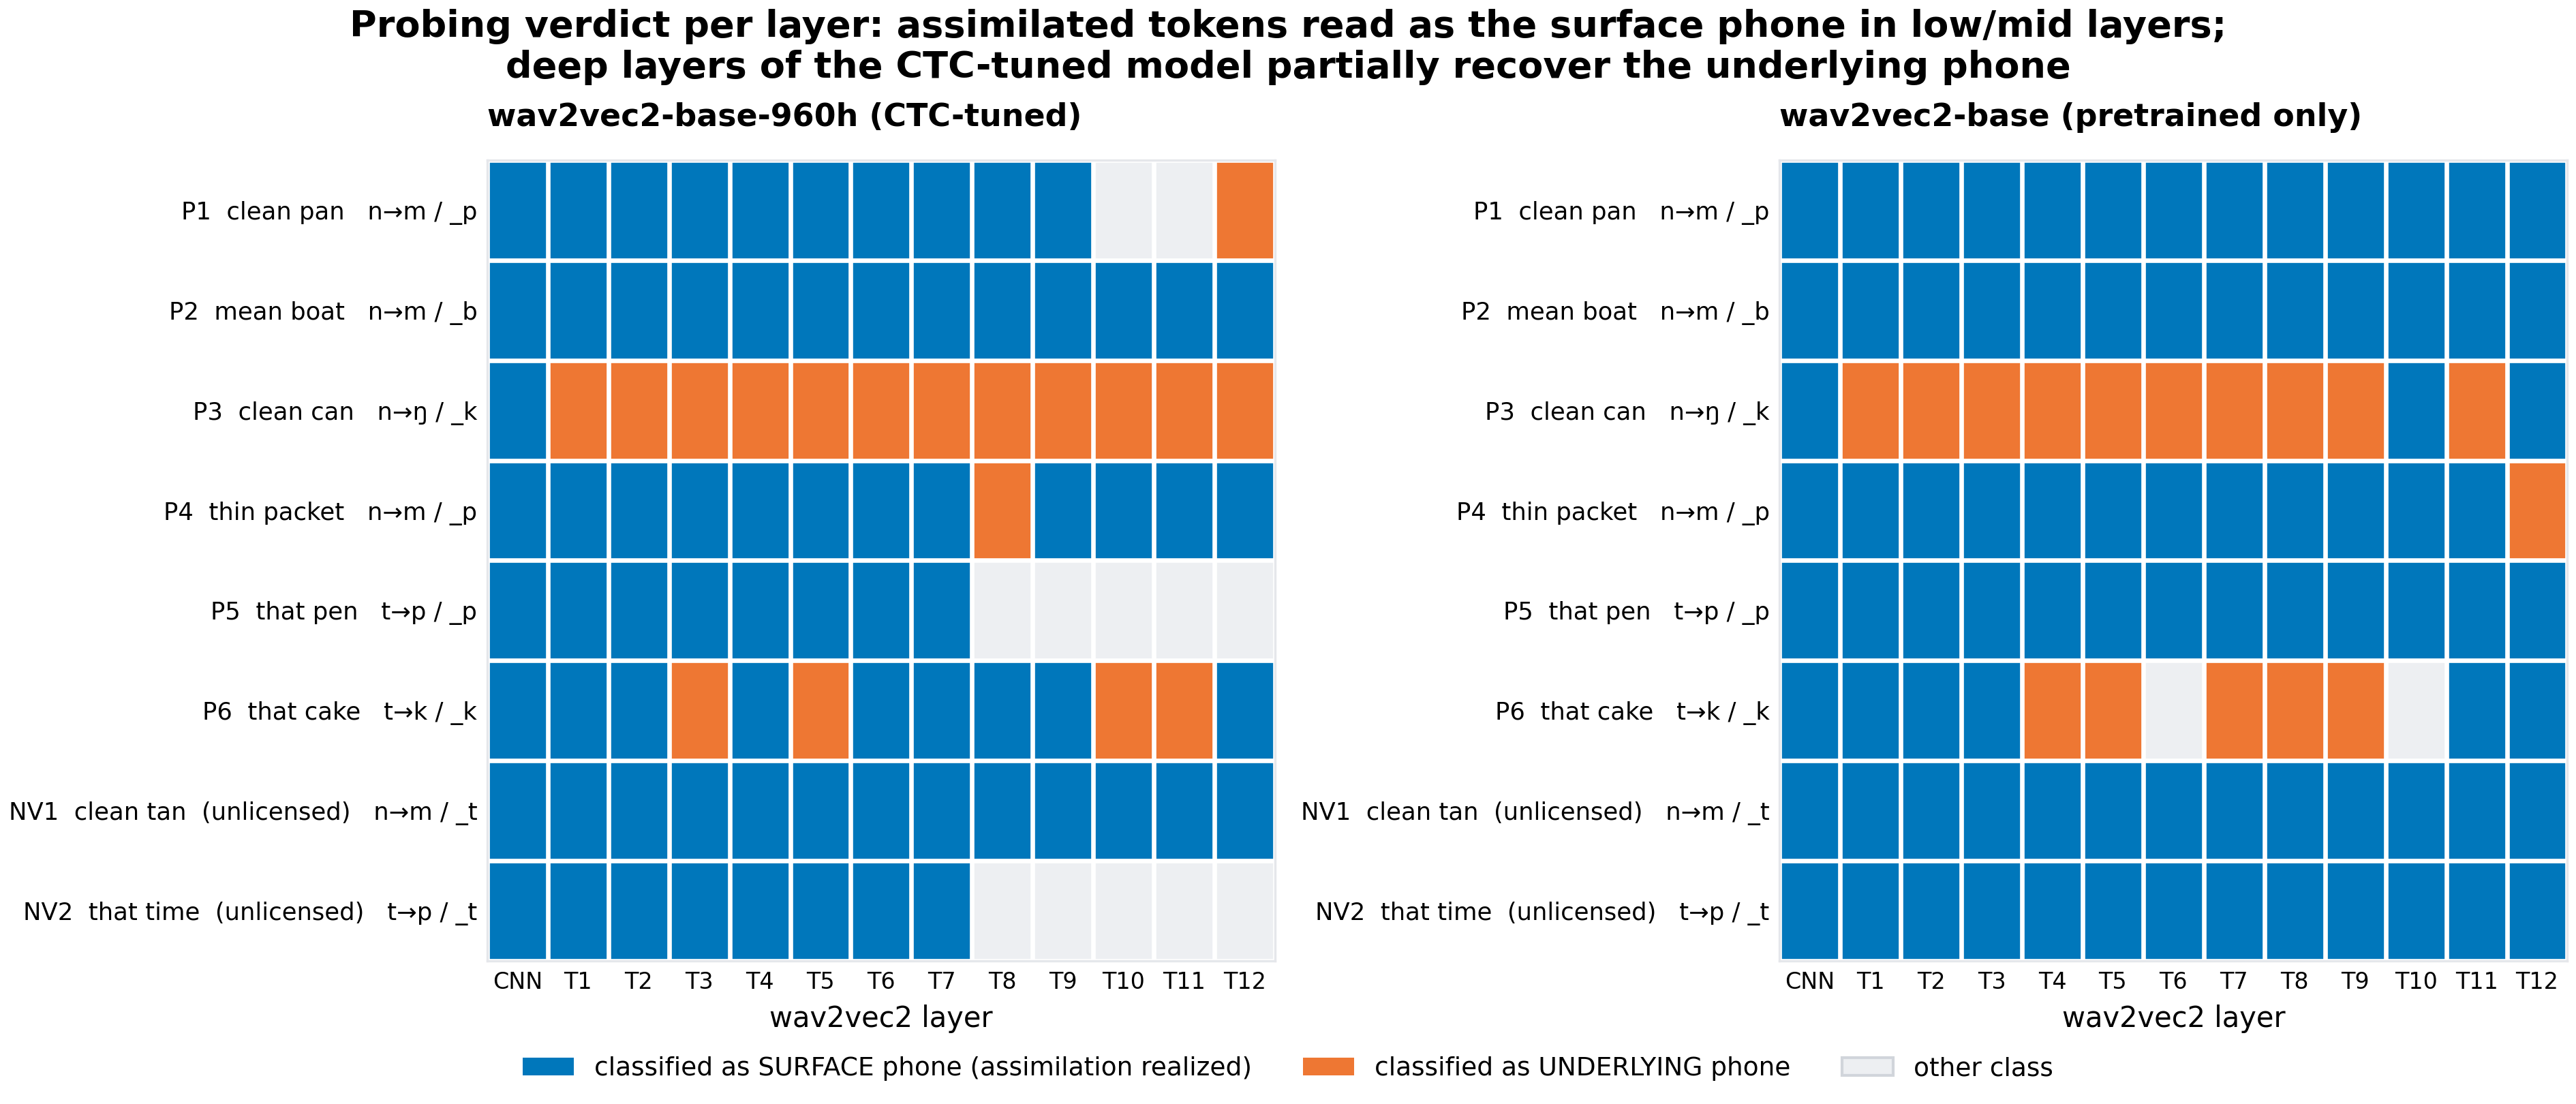
\includegraphics[width=\textwidth, max height=0.4\textheight]{fig2_classification_map.png}
\caption{Probe verdict for every assimilated/unlicensed token, layer by
layer, for both encoders (previous report). Blue = surface phone,
orange = underlying phone, gray = third class. NV1/NV2 are the
unlicensed controls.}
\label{fig:verdicts}
\end{figure}

\subsection{The letter-supervision effect}

The models part ways only in their deepest layers, and they do so in
the direction of the CTC model's training signal. For P1, the verdict
dissolves late in the fine-tuned encoder: a near tie at T8
($p_{m}=0.50$ against $p_{n}=0.27$), a flip to the third class [ŋ] at
T10 ($p=0.45$), and the underlying /n/ winning at T12 with
$p_{n}=0.52$. The self-supervised model casts the same token as /m/ in
13 of 13 layers. P5 (\emph{tha[p] pen}) shows a second flavor of the
same drift: the long homorganic [pp] closure is re-segmented as a
single strong stop whose place is reassigned to /k/ at T8--T12
($p$ up to 0.89). And the effect even reaches \emph{canonical} speech:
P2-canonical (\emph{mean boat}, underlying [n] before /b/) drifts to
/m/ in layers T7--T12 of the CTC model (underlying rate 0.46), exactly
where the training text would have taught the model that word-final
/n/ before a labial is often spelled with the labial's letter. The
self-supervised model shows none of these effects. We summarize the
pattern as a \emph{letter-supervision effect}: pairing assimilated
acoustics with underlying spellings during CTC fine-tuning installs a
late, partial, statistics-driven pull toward the underlying category,
with re-segmentation and expectation artifacts as side products.

\subsection{No licensing at the verdict level}

The unlicensed controls answer the phonological question directly.
NV1 (\emph{clea[m] tan}) is classified as /m/ in 13 of 13 layers in
both models; NV2 (\emph{tha[p] time}) as /p/ in 13/13 layers of the
base model (8/13 in the CTC model, whose late layers drift to /k/
exactly as in P5). An [m] before /t/ is represented exactly like an
[m] before /p/: neither encoder implements anything resembling an
assimilation-licensing rule. Whatever ``knowledge of assimilation''
the CTC model displays is statistical, not rule-based---a point to
which the cross-reference returns, because it is here that our
verdict-level result and Pouw et al.'s output-level result are most
instructively different.

\subsection{The P3 exception: mid-depth representations are
context-conditioned}\label{sec:p3}

P3 (\emph{clea[ŋ] can}) breaks the surface-dominance pattern from the
very first transformer layer: the assimilated [ŋ] is classified as
/n/ from T1 on, in both encoders ($p_{n}\approx0.71$ at T4), even
though its articulation is identical to the canonical [ŋ] of the
training words (a three-way contest at the CNN layer, [ŋ] 0.40 /
[m] 0.37 / [n] 0.23, resolves toward /n/). The geometry makes the
exception visible (Figure~\ref{fig:pca}): in the PCA of layer-T4
window means, every other assimilated token has crossed onto the
surface side of the place continuum, but P3's star lands next to the
/n/ cluster. Since the segment itself cannot explain the verdict
(it is bit-identical to training [ŋ]s that are read as /ŋ/), the
explanation must be the context: the lateral onset of \emph{clean} and
the velar /k/ of \emph{can}, which wav2vec2's widening receptive
fields integrate into the window representation. By mid-depth, the
encoder's ``phone'' representation is already a context-conditioned
object. This is our representational counterpart of the mechanism that
Pouw et al.'s causal interventions expose from the other side: their
heads L4H3/L5H2 \emph{write} context information into the assimilated
frames; our P3 shows the written result.

\begin{figure}[htbp]
\centering
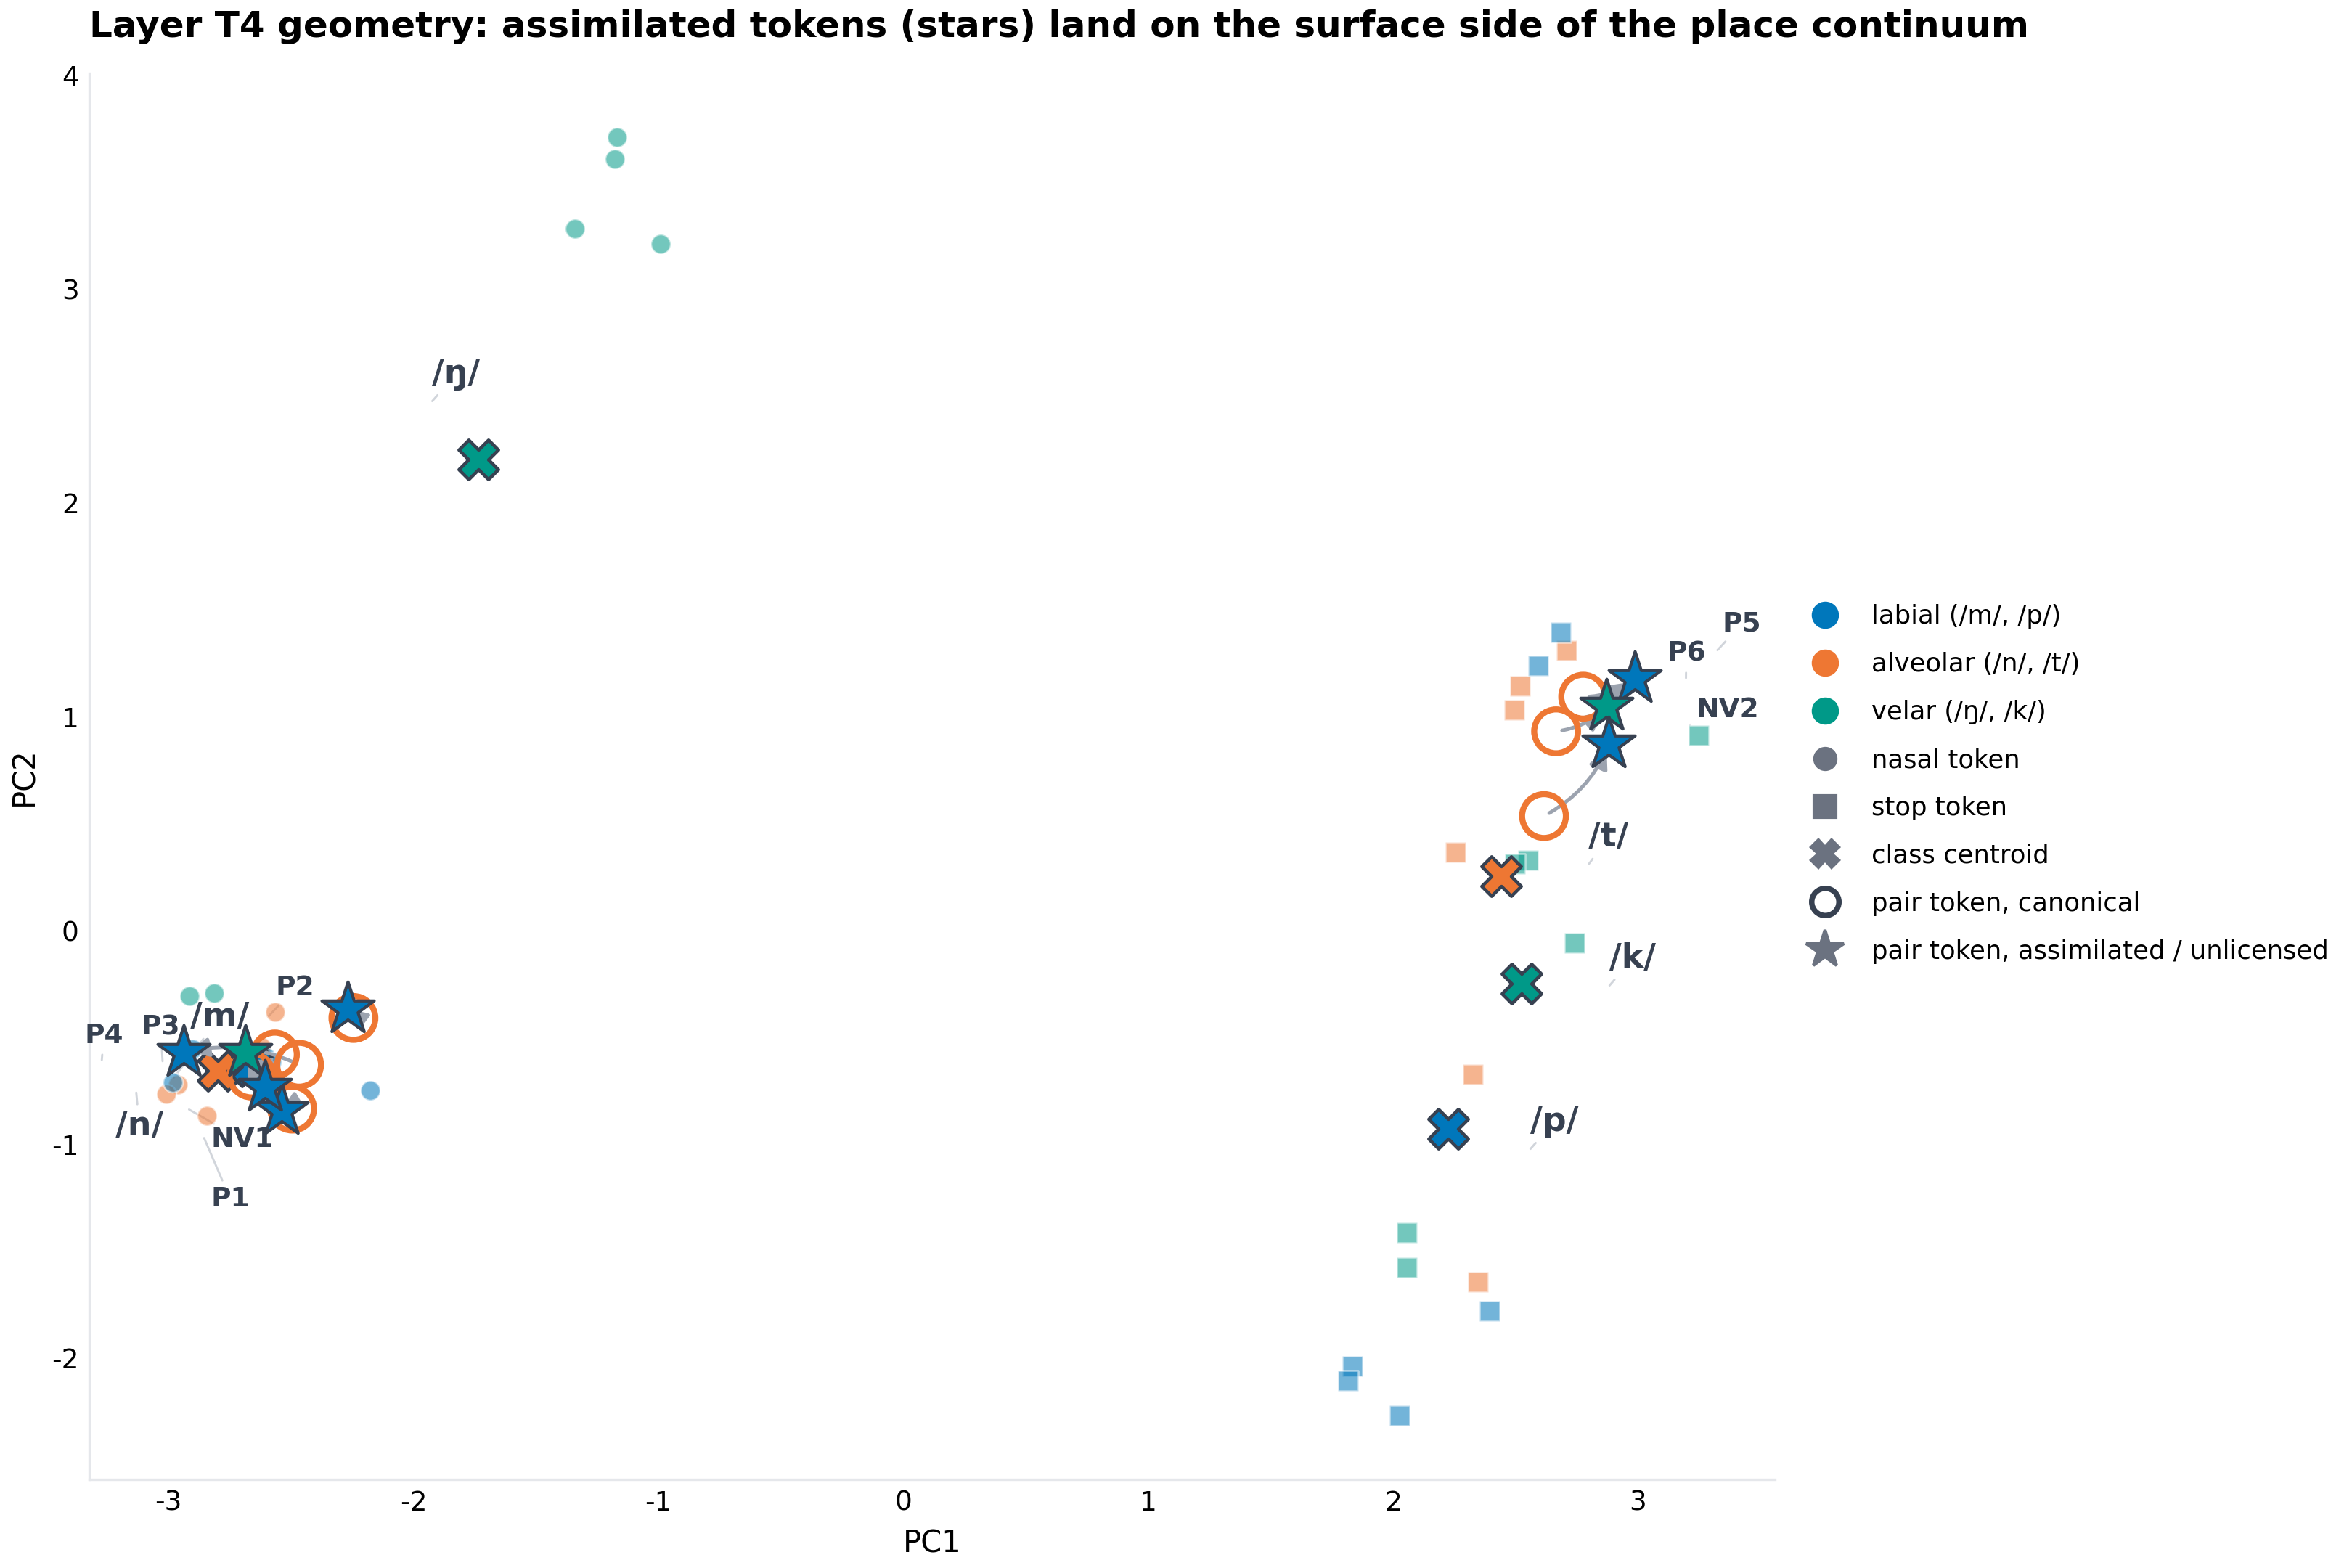
\includegraphics[width=0.85\textwidth, max height=0.4\textheight]{fig5_pca.png}
\caption{PCA of the layer-T4 window means (CTC model, previous
report). Training tokens are colored by place, circles show
pair-canonical positions, stars the assimilated/unlicensed outcomes,
arrows the canonical-to-assimilated displacement. P3's star is the one
that stays on the /n/ side.}
\label{fig:pca}
\end{figure}

% =====================================================================
\needspace{0.22\textheight}
\section{New Experiment: The Assimilation Continuum}\label{sec:lambda}
% =====================================================================

\subsection{Design}

The experiments above compare two endpoints, canonical [n] and fully
assimilated [m]. Natural speech, however, fills the space between
them~\citep{ellis2002,dilley2007}, and Section~\ref{sec:background}
argued that the intermediate regime is where acoustic and phonological
sources of information can be dissociated. This edition of the
experiment constructs that intermediate regime on the revised
reference model: the $\lam$ effect of the repository
\texttt{covtl-lambda} (v1.2.0) acts on the \emph{polar target} of the
C1 nasal of a tautosyllabic cluster,
\begin{equation}\label{eq:morph}
\theta_{C1}(\lam) \;=\; \theta_{C1} \;+\; \lam \cdot
\operatorname{wrap}\!\bigl(\theta_{C2}-\theta_{C1}\bigr), \qquad \lam
\in \bigl\{0, \tfrac{1}{8}, \tfrac{2}{8}, \dots, 1\bigr\},
\end{equation}
and the engine's own syllabic trajectory builder is re-run per degree
with the C1 node retargeted through a run-time override. The
continuum is therefore not a blend of two state sequences but a family
of \emph{re-planned gestures}: at $\lam=0$ the synthesis is bitwise
identical to the canonical cluster; at $\lam=1$ the C1 target has
reached the C2 coordinates---the place-assimilated cluster C1'C2---%
while C2 itself, the glottal block and the velum never move, and the
lips \emph{join} the gesture: this edition takes the whole CC
selector into account under $\lam$, as in the base model, whose
cluster machinery already drives the union of the two consonant
selectors. Four run-time guarantees plus three full-selector checks
are recorded per synthesis ($\lam=0$ bitwise canonical; $\theta$
equality at $\lam=1$; glottal block bitwise constant; context
outside the C1-incident arcs bitwise canonical; the recruitment
confined to those arcs; for the unlicensed frames, whose C2
selectors are subsets of sel(/n/), a verified bitwise no-op), and
all held for all 54 syntheses. The experiment is realized
for nine values of $\lam$ on six frames: the licensed pool
(\emph{clean pan}, \emph{mean boat}, \emph{thin packet}; n before the
labials /p/, /b/, /p/, a $+140^{\circ}$ target rotation) and the
unlicensed pool (\emph{clean tan}, \emph{clean can}, \emph{mean
goat}; before /t/, /k/, /g/, $+15^{\circ}$ to $+75^{\circ}$)---the
same licensed-versus-unlicensed contrast that separates Pouw et al.'s
conditions. The two pools differ in exactly the C2 of the
cluster---the same minimal contrast that separates their viable from
their unviable condition. The ground truth is gestural, not acoustic
(Figure~\ref{fig:curves}a): the rotation is carried by the jaw and
the tongue body (over P1, jaw angle $-2.34 \to -3.28^{\circ}$,
tongue-body x $3.96 \to 2.51$\,cm, y $0.20 \to 0.66$\,cm), while the
velum stays \emph{bitwise constant} along every continuum and the
lips are recruited in proportion to $\lam$ on the labial-C2 frames
(lip opening at the C1 target point of P1: $0.61 \to 0.46 \to 0.16
\to 0.00$\,cm at $\lam = 0/0.5/0.75/1$, with protrusion rising to
the base model's own labial value)---the full CC selector realizes
the interpolated target, so the assimilated C1 is a nasal whose
gesture \emph{becomes} C2's, closure included, degree by degree.
Each of the 54 stimuli was synthesized with the same engine,
resampled and normalized exactly like the base material, passed
through both encoders, and classified by the unchanged nasal probe
instrument (leave-one-sentence-out accuracies identical to the
stage-1 report), so the continuum is measured by the same probes as
the endpoints.

Two facts secure the validity of the new material. First, the four
run-time guarantees and three full-selector checks above are
structural, checked per synthesis
against the engine's own canonical output---$\lam=0$ is \emph{by
construction} the canonical cluster, not a re-synthesis of it, so no
endpoint anchoring against the stage-1 items is needed or meaningful
(the stage-1 dotted citation forms differ from the cluster by design;
the machine-readable distance between the tiers, up to $0.86$ in
$P(\mathrm{n})$, is reported as the coarticulation signature of the
tautosyllabic cluster). Second, all nine degrees of all six frames
were probed in a single run with one instrument, so every
cross-section comparison of this document---anchors, production
degrees, dose-response---is a slice of one experiment rather than a
family of re-runs, and the leave-one-out accuracies of the stage-1
report remain the honest generalization measure.

\subsection{Where the category boundary went}

Figure~\ref{fig:heatmap} maps the probe probability of the underlying
/n/ over the layer $\times$ $\lam$ plane, for both encoders, the
licensed frame P1 against the unlicensed velar frame NV3. Read first
along the $\lam$ axis at the phone-encoding layer T4
(Figure~\ref{fig:curves}b): the probability of /n/ \emph{never falls
below 0.5 anywhere on the revised continuum}. The per-frame T4 minima
stay between $0.46$ and $0.84$, the pooled pool-level curves never
cross, and the category boundary that anchored the previous edition's
reading ($\lam^{*} \approx 0.7$--$0.9$) does not exist. Three facts
deserve the reader's attention. First, the boundary's disappearance is
articulatory, not statistical: the motor blend of the previous
editions closed the lips inside the C1 window, producing real [m]
acoustics that the phone code tracked; the target-level rotation
moves the jaw and the tongue, and the resulting acoustics never leave
the /n/ basin. The full-selector condition of this edition closes
the lips again---in proportion to $\lam$, reaching the base model's
own labial closure at $\lam=1$---and the boundary still does not
return: the encoder is not merely tolerating an incomplete gesture;
it keeps the underlying reading through a completed labial closure
whose tongue keeps aiming at the rotated target. Second, what T4 tracks instead is the \emph{coarticulation
cleanup}: on the velar-C2 frames the probability of /n/ rises
monotonically with $\lam$ (NV3: $0.81 \to 0.90 \to 0.95$; pooled
unlicensed $\rho(\lam, P(\mathrm{n})) = +0.90$ at T4), because the
canonical cluster's murmur is labial-coarticulated---the CNN reads it
as /m/-ish at $\lam=0$ ($P(m) = 0.54$ pooled licensed)---and rotating
the C1 target away from the labial blend moves the murmur toward the
trained /n/ centroid. The continuum is graded, as \citet{ellis2002}
describe articulatorily, but its gradient at the phonetic layers is a
coarticulation gradient, not an assimilation gradient. Third, and most
important for the cross-reference: the only categorical surface event
of the continuum lives at the deepest CTC layers and the very end of
the rotation---at $\lam=1$ the licensed pool's deep cells read [m]
(pooled $P(\mathrm{m})$ at T10--T11 of the CTC model: $0.57$--$0.66$)
---and the full-selector condition reallocates it: the crossing is
carried by P2 and P4, whose cluster context produced it already at
$\lam=0$, while P1, whose lips now close, \emph{loses} its endpoint
crossing (T10--T11: $P(\mathrm{m}) = 0.24/0.09$ against
$0.44/0.53$ with the lips blocked)---so any context sensitivity the
encoders display is confined to exactly the layers where letter
supervision lives and is driven by the cluster context, not by the
surface closure, and never by the phone code that sets boundaries.

\begin{figure}[htbp]
\centering
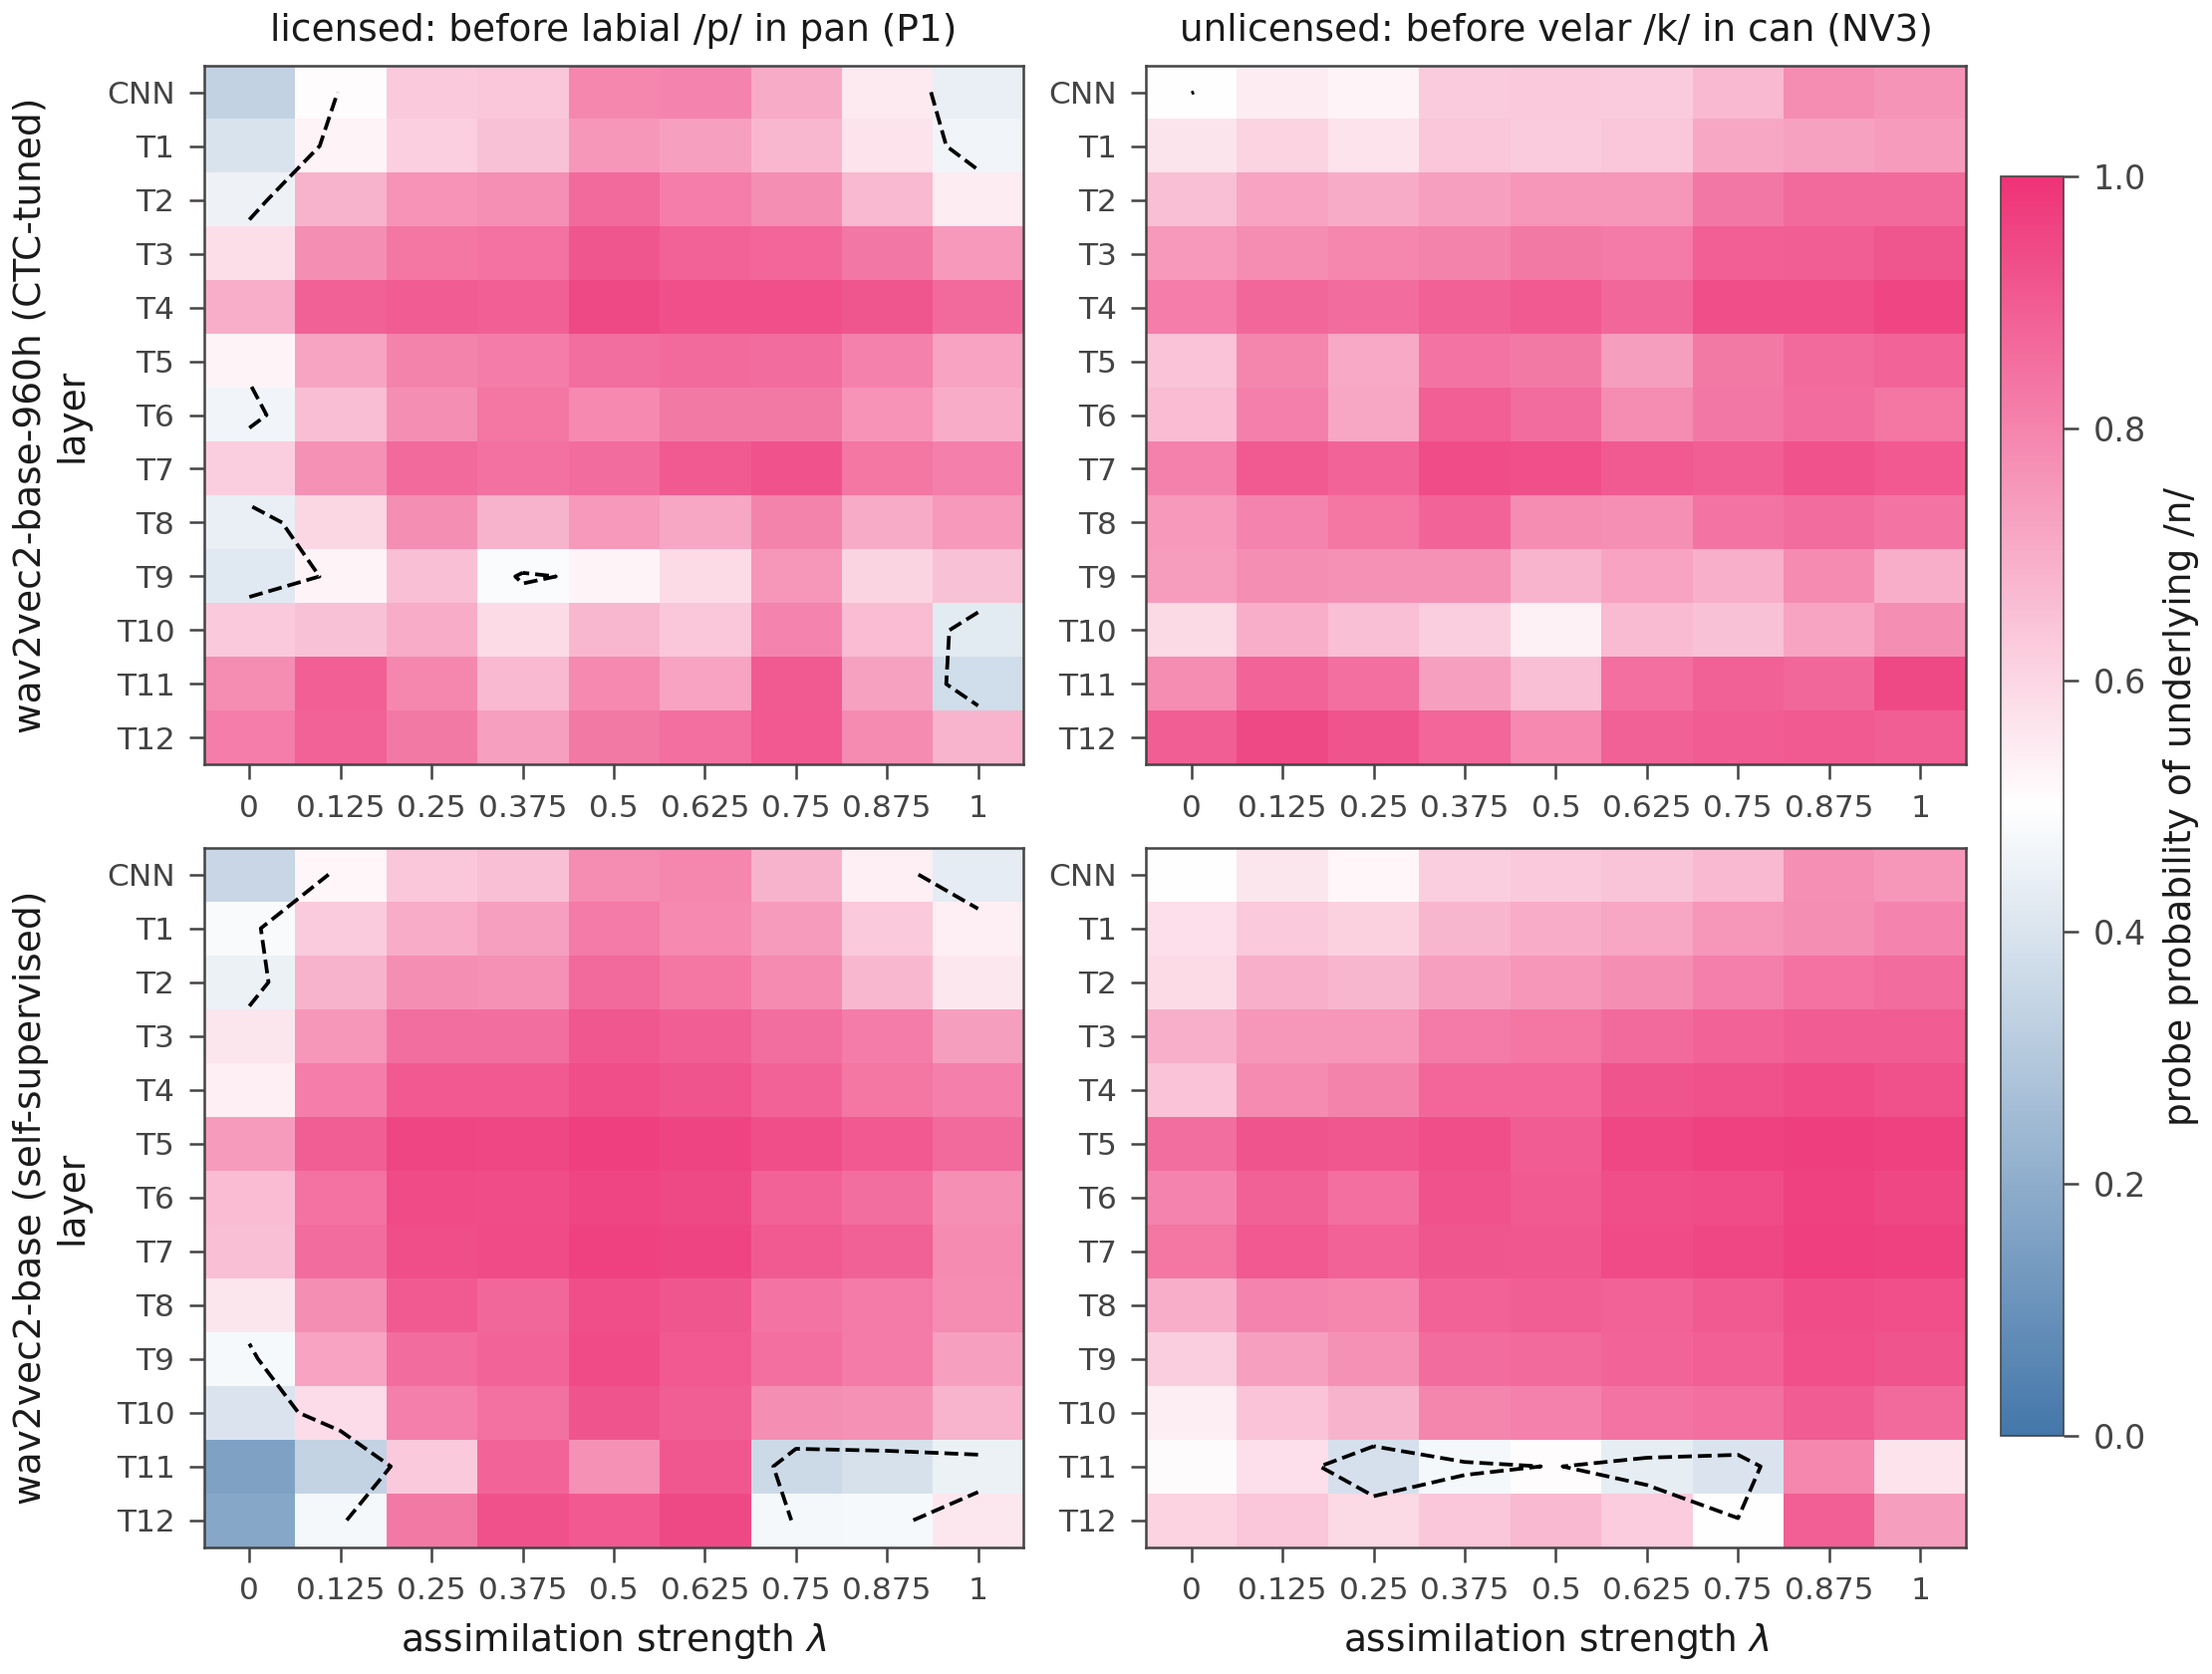
\includegraphics[width=\textwidth, max height=0.42\textheight]{figL1_continuum_heatmap.png}
\caption{The assimilation continuum, probed. Color encodes the nasal
probe's probability of the underlying /n/ for every layer (CNN, T1--T12)
and every target-rotation strength $\lam$ (Eq.~\eqref{eq:morph}), in
the licensed frame P1 (\emph{clean pan}, labial C2) and the
unlicensed velar frame NV3 (\emph{clean can}), for both encoders. The
dashed black contour marks $P(/n/)=0.5$ where it exists---at the
phonetic layers it does not: the continuum has no category boundary,
and in the licensed column the contour now survives only
transiently (P1, around $\lam \approx 0.4$ and at the T10--T11
endpoint of the deepest layers); the sustained endpoint crossing
lives on P2/P4, outside this figure.}
\label{fig:heatmap}
\end{figure}

\begin{figure}[htbp]
\centering
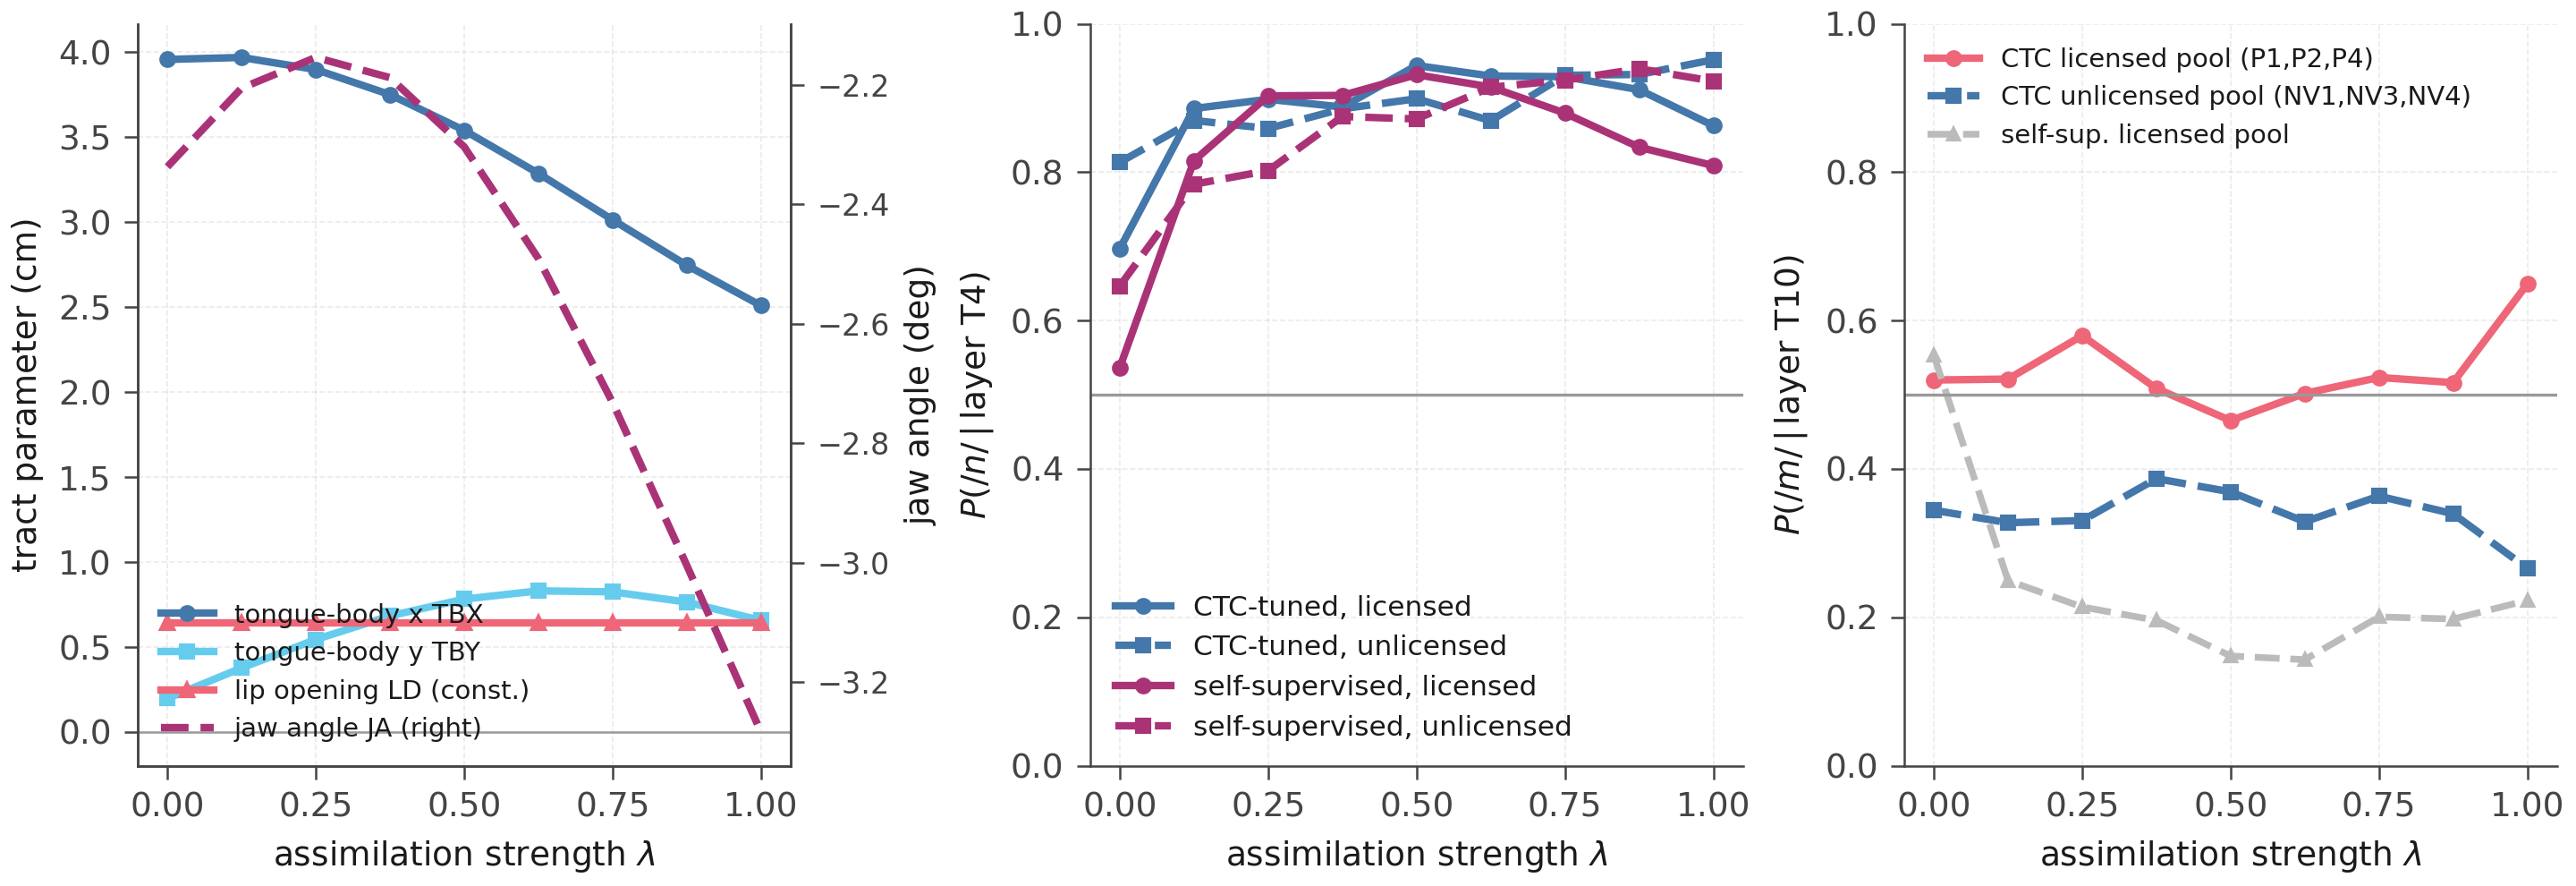
\includegraphics[width=\textwidth, max height=0.36\textheight]{figL2_boundary_curves.png}
\caption{Reading the continuum. (a) Articulatory ground truth at the
midpoint of the C1 window (P1): the gesture carriers vary with
$\lam$---tongue-body x and y drift, the jaw angle (right axis)
drops---and the lip opening joins the gesture with weight $\lam$
(the full CC selector; the dotted vertical marks $\lam=0.5$). (b) Probability of the underlying /n/ at layer T4
as a function of $\lam$: every curve stays high; the velar frame NV3
rises with $\lam$ (coarticulation cleanup) and no curve crosses 0.5.
(c) The late-layer [m] surface: $P(/[m]/)$ at layer T10 of the CTC
model, licensed pool (mean of P1, P2, P4) against the unlicensed
pool---the assimilated reading is a late-layer, labial-C2 phenomenon,
present already at $\lam=0$ on P2/P4 and indifferent to the recruited
closure of P1, absent from the unlicensed pool and from the
self-supervised model.}
\label{fig:curves}
\end{figure}

\subsection{A labial-context reading in the deep CTC layers}

The heatmaps' bottom rows are where the two columns finally separate,
and only in the CTC-tuned model. Figure~\ref{fig:curves}c reads this
as $P(/[m]/)$ at T10 for the licensed pool against the unlicensed
pool, degree by degree. In the deepest CTC layers (T10--T11) the
licensed pool carries a [m] reading that is \emph{unidirectional} in
$\lam$: it is already present at $\lam=0$ (pooled $P(m)$ at T10 of
$0.46$--$0.54$, driven by P2 and P4), and the full-selector condition
shows how gesture-blind it is: with the lips blocked (v3.0) the
rotation sharpened P1's reading ($0.24 \to 0.44$ at T10, crossing at
T11); with the lips \emph{recruited}---a true labial closure through
most of the C1 window---P1's reading reverts to its baseline
($0.24 \to 0.24$ at T10, $P(\mathrm{m}) \leq 0.09$ at T11) while
P2/P4 keep theirs. The model has learned that a nasal in a
tautosyllabic cluster before a labial is where /n/ is often spelled
with the labial's letter, and its deepest layers read that context as
[m] \emph{regardless of the gesture---and regardless of the closure}:
at $\lam=0$ the C1 is a canonical alveolar closure, at $\lam=1$ its
lips are closed on the labial place, and the reading is the same
wherever the context already produced it. This is the continuum
generalization of the P2-canonical attraction reported in the probing
campaign, and it is \emph{not} a compensation effect: it suppresses
the underlying interpretation in exactly the context where
compensation would enhance it. The decisive frame is P4 (\emph{thin
packet}): it contains no /m/ segment anywhere, yet its T10 reading is
[m] along the whole continuum ($P(m)$ up to $0.82$ at $\lam=1$)---the
reading is carried by the cluster context, not by the token's own
phonetics. The self-supervised model shows none of this
(licensed-pool T10 $P(m)$ stays at or below $0.30$ beyond $\lam=0$),
and its $\lam=0$ licensed deep cells carry only the known late-layer
quirk of the canonical token (a T11--T12 drift that recovers one
half-step into the continuum). The modulation is therefore cleanly
unidirectional and layer-consistent only in the letter-tuned model,
and we attribute it to letter supervision, like the underlying drift
itself. We emphasize what the effect is \emph{not}: across the whole
54-item continuum the CTC model's verdicts flip toward the surface
reading only at T10--T11 of the licensed frames at the high
degrees---never at the phonetic layers, never in the unlicensed pool
(NV1 and NV3 return /n/ at 13 of 13 layers at every $\lam$), and the
velar drift of NV3/NV4 never surfaces as the trained velar nasal
($P(\text{ŋ}) \leq 0.18$ for NV3 at every layer and degree).
Elsewhere the context moves probabilities, not classifications, and
only in layers adjacent to the letter output.

% =====================================================================
\needspace{0.22\textheight}
\section{The Cross-Reference: Our Results $\times$ Pouw et al.}\label{sec:cross}
% =====================================================================

We now perform the croisement the title announces: dimension by
dimension, what do the two programs agree on, what do they add to each
other, and where do they genuinely differ? Table~\ref{tab:cross}
summarizes the comparison; the paragraphs below justify each row.

\begin{table}[htbp]
\centering
\footnotesize
\caption{Systematic cross-reference between Pouw et al.\ (2024) and the
present experimental program. C = convergent, X = complementary,
D = divergent.}
\label{tab:cross}
\begin{tabularx}{\textwidth}{@{}l Y Y c@{}}
\toprule
Dimension & Pouw et al.\ (2024) & Present program & \\
\midrule
Model set & wav2vec2-base-960h; base checked in a footnote &
base-960h and base as the main factorial design & C+X \\
Stimuli & natural speech, complete assimilation, 3 conditions $\times$
carriers & VTL synthesis, frame-aligned causal pairs, unlicensed
controls, 9-step articulatory continuum & X \\
Default encoding & probing: no-compensation cases stay surface at all
layers & $\approx$80\% surface across 156 token-layer decisions & C \\
Late-layer shift & probing: compensated cases shift surface
$\to$ underlying in final layers; pretrained model converges instead &
P1 drifts to /n/ at T12 ($p{=}0.56$) in the CTC model; base: a single
T11 flip & C \\
Phonological context & ASR: compensation higher in viable than
unviable contexts ($\approx$40\% residual) & verdicts: no licensing
whatsoever (NV controls: /n/ at 13/13 layers at every $\lam$);
continuum: no T4 boundary at all; the deep layers read [m] on
labial-C2 clusters (P4, with no /m/ segment) & X \\
Deep-layer context effect & not separable from decoding at the output
level & unidirectional labial-context reading at T10--T11: present
at $\lam=0$ (pooled $P(m) \approx 0.5$ licensed), indifferent to
the recruited lip closure, CTC model only & X \\
Lexical knowledge & output level: non-word vs.\ real-word asymmetry;
\emph{wept}, \emph{playing} over-rides & excluded by design (probing
reads representations, no decoding); P3 shows context-lexical
conditioning of representations & X \\
Semantic context & no effect on the model (unlike humans) & not tested
& (gap) \\
Mechanism & interchange interventions: early MLPs at the context phone;
heads L4H3/L5H2 move the cue & tract-level intervention: causal delta
localizes the divergence in time; depth amplifies it & X \\
Gradience & excluded by design (complete assimilation only) & the
continuum: no assimilation boundary; a graded coarticulation cleanup
(velar pools $\rho(\lam, P(\mathrm{n}))$ up to $+0.98$ at T4) & X \\
\bottomrule
\end{tabularx}
\end{table}

\paragraph{Convergences.}
Three results line up so cleanly that the two programs can be said to
have measured the same object. The first is surface dominance: their
probes read the assimilated consonant as its surface phone at every
layer whenever the model's output failed to compensate, and our
verdicts read the surface phone in roughly 80 percent of token-layer
decisions---despite completely different material (natural recordings
vs.\ synthesis), different probe families (binary TIMIT-trained
logistic regression vs.\ three-way probes trained on our own synthetic
canonicals), and different frame-selection rules. When the waveform
says [m], the first dozen layers of wav2vec2 say [m]. The second
convergence is the late-layer underlying shift restricted to the CTC
model: their compensated cases migrate to the underlying phone in the
final layers, their pretrained checkpoint (footnote~5) converges
instead of diverging, and our factorial design turns that footnote into
a systematic contrast---the same drift, present in the letter-tuned
model, absent in the self-supervised one. The third is the refusal of
the phone code to implement licensing: their unviable compensation
survives only at the output level, and our unlicensed controls never
recover the underlying phone at the representation level in any layer
of either model.

\paragraph{Complementarities.}
The programs fill each other's blind spots so precisely that the
combination is more informative than either alone. Pouw et al.\ measure
\emph{behavior} (transcriptions) and therefore include everything the
decoding stage contributes---lexical override of non-words like
\emph{cleam}, bigram statistics, the character prior. Our probes
measure \emph{representations} at fixed articulatory ground truth and
exclude decoding altogether. The instructive case is the unviable
condition: their model still ``compensates'' about 40 percent of
unviable non-word stimuli at the output, while our unlicensed [m]
before /t/ never recovers /n/ in the representations---not even
probabilistically at T4, not even at $\lam$ values where the token is
mostly [n]. Read together, the two results localize the unviable
compensation in the decoding/lexical stage, not in the phone
representation: the encoder hands the decoder an honest [m], and the
decoder, disliking the non-word \emph{cleam}, writes \emph{clean}. The
continuum adds a finer instrument still: the phone code's category
boundary is \emph{context-free} (identical before /p/ and /t/), while
the deep CTC layers' underlying-probability is \emph{context-sensitive}
(bidirectionally so), which no endpoint-only design could have
revealed. Conversely, their causal interchange interventions give what
our design cannot: the \emph{components} (early MLPs, heads L4H3 and
L5H2) that move the context cue into the assimilated frames, whereas
our causal delta gives what theirs cannot: the \emph{time course} and
depth profile of a single controlled articulatory change, showing the
divergence confined to the manipulated window and amplified
monotonically with depth. Their Whisper comparison and our two-model
factorial both point at the training objective as the carrier of
``compensation knowledge,'' from opposite directions.

\paragraph{Divergences and open contrasts.}
Only one dimension shows a real tension, and it is a tension of
interpretation rather than of fact. Pouw et al.'s headline is that
wav2vec2 exhibits human-like, context-sensitive compensation; ours is
that the context sensitivity lives in layers adjacent to the letter
output, is probabilistic rather than categorical, and is absent from
the self-supervised checkpoint---which their own footnote~5
corroborates. The disagreement is thus about how much weight the word
``compensation'' should carry when the effect neither flips
classifications nor survives without letter supervision. The honest
summary is that the two studies bracket the phenomenon: at the output,
with the lexicon in the loop, wav2vec2 behaves as a partial
compensator; at the representation level, with the lexicon out of the
loop, it behaves as an acoustic veridicalist with a supervised,
statistical late correction. One contrast remains genuinely untested:
semantic context, which their Experiment~3 showed the model ignores;
our material (two-word sentences, no biasing contexts) cannot speak to
it.

% =====================================================================
\needspace{0.22\textheight}
\section{A Two-Stage Account of Assimilation Processing}\label{sec:twostage}
% =====================================================================

The synthesis of the two programs is best stated as a two-stage
architecture, schematized in Figure~\ref{fig:twostage}.

\paragraph{Stage 1: an acoustic, context-free phone code
(CNN--T6).}
The early and middle layers of wav2vec2---both checkpoints
alike---encode the consonant as what it acoustically is. On the
revised continuum this stage is \emph{boundary-free}: the target-level
rotation changes the acoustics so little that the probability of the
underlying /n/ never crosses 0.5 at any degree of any frame, and what
the phonetic layers track is the coarticulation of the canonical
cluster (the CNN's /m/-ish baseline) and its cleanup under the velar
rotation ($\rho$ up to $+0.98$). This stage is surface-veridical,
phonetically graded, and phonologically blind. Its human analogue is
the pre-lexical, signal-borne stage that uses residual acoustic traces
\paragraph{Stage 2: a supervised labial-context reading
(T7--T12).}
In the CTC-tuned model only, the deepest layers install a statistical
reading shaped by letter supervision: a nasal in a tautosyllabic
cluster before a labial is read toward the labial's letter, [m],
regardless of the gesture (the expectation effect at $\lam=0$ and the
surface reading at $\lam=1$ are one and the same effect, present on
P2/P4 at the baseline, and the full-selector condition shows it is
closure-blind: recruiting P1's lips removes its endpoint sharpening
and leaves the P2/P4 reading untouched), and
its aggregate result is a licensed-pool \emph{deficit} in underlying
verdicts---now on both listeners ($-20.5$ and $-17.9$ points at
$\lam=1$, the two significant licensed--unlicensed contrasts we
measure)---the opposite sign to the
viable-over-unviable advantage that Pouw et al.\ measured behaviorally.
This stage is context-sensitive, unidirectional, probabilistic,
and---on the evidence of the self-supervised checkpoint and of Pouw et
al.'s footnote---a product of training on underlying spellings rather
than of self-supervised structure learning. Its circuit substrate, on
the evidence of the interchange interventions, is already in place by
layers 4--5, where attention heads gather the context phone and early
MLPs write it into the target frames.

\begin{figure}[htbp]
\centering
\begin{tikzpicture}[
  stage/.style={draw, rounded corners=3pt, text width=6.1cm,
                minimum height=3.4cm, align=left, font=\small},
  arr/.style={-{Stealth[length=5pt]}, thick, gray!70}
]
\node[stage, fill=blue!5] (s1) {\textbf{Stage 1: acoustic phone code}
  \newline CNN -- T6 (both checkpoints)
  \newline\small $\bullet$ surface-veridical: [m] is /m/
  \newline\small $\bullet$ boundary-free on the target continuum
  \newline\small $\bullet$ tracks cluster coarticulation, not
  assimilation};
\node[stage, fill=orange!8, right=2.2cm of s1] (s2)
  {\textbf{Stage 2: supervised reading} \newline T7 -- T12
  (CTC-tuned only)
  \newline\small $\bullet$ labial-context: n\,+\,labial reads [m]
  \newline\small $\bullet$ gesture-blind: same at $\lam\!=\!0$
  and $\lam\!=\!1$
  \newline\small $\bullet$ probabilistic: verdicts flip only at
  T10--T11, licensed, high $\lam$};
\draw[arr] (s1) -- node[above, font=\footnotesize, text=gray]
  {context cues} (s2);
\end{tikzpicture}
\caption{The two-stage account. The division of labor emerges from the
cross-reference: an acoustic, context-free phone code, common to both
checkpoints, that holds the underlying /n/ across the whole gestural
rotation, and a late, letter-supervised, labial-context reading present
only in the CTC-tuned model. The context cues that stage~2 exploits are
written into the target frames by the circuit that Pouw et al.'s
interchange interventions localize: early MLPs and attention heads in
layers 4--5.}
\label{fig:twostage}
\end{figure}

\paragraph{What the account buys.}
The two-stage account explains, in one stroke, every empirical
regularity this document has assembled. It explains why surface
dominance is the default (stage 1 does the encoding) and why the
underlying drift is late, partial, and pair-specific (stage 2 is a
statistical correction, not a rule). It explains why unlicensed
assimilations are never compensated in the representations (stage 2
moves probabilities, and only where training statistics support them)
yet are compensated 40 percent of the time at the output (the decoding
stage adds the lexicon). It explains why the phone code has no assimilation
boundary on the revised continuum (stage 1 tracks acoustics, and the
target rotation barely changes them) while the deep-layer probability
is context-sensitive (stage 2 reads the cluster context, not the
gesture). And it aligns the machine with the human
literature in a specific, testable way: human compensation also has an
early, signal-driven component that exploits incomplete-assimilation
traces~\citep{gaow2002} and a later, knowledge-based component that
checks phonological viability~\citep{gaskell1996,mitterer2003}, with
the timecourse of the two stages measurable in
EEG~\citep{mitterer2003}. The machine's stage 2 differs from the
human's in its provenance---letter statistics rather than whatever
installs phonological knowledge in humans---and in its indifference to
semantics, which Pouw et al.'s Experiment~3 demonstrated and which no
amount of probing on two-word sentences could rescue.

% =====================================================================
\needspace{0.25\textheight}
\section{Reproducibility: The Experiment Kit}\label{sec:repro}
% =====================================================================

Every number, verdict, and figure in this document is traceable to a
machine-readable artifact, and every artifact is regenerable from the
released scripts. The release is organized as an \emph{experiment
kit}: one self-contained directory that holds the data of both
experimental stages, the tooling that produced them, and the complete
source of this document. A reader can therefore move in both
directions---from any claim back to the measurements that support it,
and forward to a fresh replication on their own machine. The kit is
deliberately compact (about 25\,MB uncompressed): the only components
not shipped are the two wav2vec2 checkpoints and the per-sentence
feature caches (a few hundred megabytes), both of which are recreated
automatically on first use. This section presents the layout, walks
through the pipeline script by script, gives the exact commands for a
full re-run, and lists the checks that make a re-run verifiable.

\subsection{Layout}

Table~\ref{tab:kit} maps the kit to the concepts of
Sections~\ref{sec:program} and~\ref{sec:lambda}. Two conventions hold
throughout. First, every script resolves its inputs and outputs
relative to the kit root (the parent directory of \sampa{repro/}), so
the kit can be unpacked anywhere; the environment variable
\sampa{COVTL\_KIT\_ROOT} overrides the root for non-standard layouts.
Second, every result file is plain JSON with the layer names
(\sampa{CNN}, \sampa{T1}--\sampa{T12}) and the item labels spelled
out, so every number in this document can be checked in a text editor,
without executing any code. The compiled document itself ships at
the kit root as \path{nasal_place_assimilation_synthesis.pdf}.

\begin{table}[htbp]
\centering
\small
\caption{The experiment kit.}
\label{tab:kit}
\begin{tabularx}{\textwidth}{@{}l X@{}}
\toprule
Path & Contents \\
\midrule
\sampa{README.md} & navigation guide and quickstart \\
\sampa{repro/} & the tooling: the eight scripts of
Table~\ref{tab:scripts}, plus \sampa{requirements.txt} \\
\sampa{work/base/} & the 52-item synthesis base: per item the SAMPA
text, the 400\,Hz tract-and-glottis sequence, the polar control-plane
state, and the 44.1\,kHz waveform \\
\sampa{work/results/} & stage-1 probing outputs, per model: LOSO
accuracies, classification verdicts with probabilities, causal delta,
timecourses; plus cross-model summary statistics \\
\sampa{work/lambda/} & the continuum experiment: the 54 tract files
(\sampa{tracts/}) and 54 waveforms (\sampa{wavs/}) of the campaign
(six frames $\times$ nine degrees), the per-frame morph meta-data, the
synthesis provenance with the four run-time guarantees and per-file
SHA-256 hashes (\sampa{synth\_meta.json}), and the per-layer probe
outputs (\sampa{results.json}) \\
\sampa{work/lambda075/}, \sampa{work/lambda0625/} & the production-
degree blocks: byte-identical subsets of the continuum (18 and 24
items) with their condition statistics \\
\sampa{work/legacy\_lipblocked/},
\sampa{work/legacy\_motorblend/}, \sampa{work/legacy\_unconfined/} &
the superseded $\lam$ tiers (v3.0 blocked-lip campaign, byte-identical;
v2.1 confined motor blend; v2 unconfined dotted), with the
machine-readable comparisons
(\sampa{revision\_comparison\_v31.json},
\sampa{revision\_comparison\_v30.json},
\sampa{correction\_comparison.json}) \\
\sampa{figures/} & the four figures of this document (PNG, 300\,dpi) \\
\sampa{latex/} & full document source: \sampa{main.tex}, the cover,
and the figures \\
\bottomrule
\end{tabularx}
\end{table}

\subsection{The tooling}

Table~\ref{tab:scripts} lists the eight scripts in execution order,
with their roles and measured runtimes on a laptop-class CPU. Three
design properties deserve emphasis. First, the corpus is \emph{data,
not code}: the 52 sentences, their canonical and assimilated
variants, and the licensing labels live in one declarative module
(\sampa{sentence\_base.py}) that both the synthesis and the probing
scripts import, so the corpus definition cannot drift between stages.
Second, the engine modification of Section~\ref{sec:program} is a
dedicated, idempotent patch script that asserts exactly one match
before editing the engine's phoneme table and leaves its provenance
comment inside the edited source; the whole change is three lines.
Third, the continuum experiment of this edition runs on the reference
$\lam$ model extended by the kit's own additive module
(\sampa{repro/morphing\_fullsel.py}: under $\lam$ the whole CC
selector is taken into account): the pinned engine checkout
(covtl-pipeline \texttt{1d15ed7} + the committed corrections series)
with the \texttt{covtl-lambda} v1.2.0 patch applied, its 53-test
suite green; the 54 syntheses carry the model's four run-time
guarantees plus the three full-selector checks, and the
probing stage reuses the stage-1 instrument unchanged (LOSO curves
identical), so continuum and endpoints are measured alike.

\begin{table}[htbp]
\centering
\footnotesize
\caption{The tooling, in execution order. Runtimes are for a
laptop-class CPU; the feature stages download the two checkpoints on
first use.}
\label{tab:scripts}
\begin{tabularx}{\textwidth}{@{}l X l@{}}
\toprule
Script & Role & Time \\
\midrule
\sampa{patch\_N.py} & engine fix: velar closure for \sampa{N} (edit of
the covtl-pipeline phoneme table) & s \\
\sampa{sentence\_base.py} & declarative corpus definition (52 items,
four groups) & s \\
\sampa{build\_base.py} & synthesize the base: SAMPA $\to$
tract/polar/wav per item & $\approx$5\,min \\
\sampa{extract\_features.py} & wav2vec2 features: 16\,kHz audio $\to$
13 hidden states $\times$ 2 models, one \sampa{.npz} per sentence (not
shipped) & $\approx$30\,min \\
\sampa{run\_probing.py} & LOSO probes, verdicts, probabilities,
cosine statistics, causal delta, timecourses & $\approx$2\,min \\
\sampa{figures.py} & stage-1 figures (two of them reappear as
Figs.~\ref{fig:verdicts} and~\ref{fig:pca}) & s \\
\sampa{make\_results.py} & slice the campaign probing output into the
kit blocks (continuum + the two production-degree subsets, asserted
byte-identical) & s \\
\sampa{note\_stats.py}, \sampa{pouw075\_stats.py},
\sampa{pouw0625\_stats.py} & the statistics of the anchors, the
production degrees, and the nine-degree dose-response & s \\
\sampa{lambda\_figures.py}, \sampa{note\_figure.py} & continuum and
note figures (Figs.~\ref{fig:heatmap} and~\ref{fig:curves} among
them) & s \\
\bottomrule
\end{tabularx}
\end{table}

\subsection{Rerunning the experiment}

A complete replication from a clean machine reduces to the command
sequence below. Steps~1--3 rebuild the stage-1 material from scratch;
they can be skipped if the shipped \sampa{work/base/} is trusted, in
which case the replication starts at step~4 and needs about fifteen
minutes of compute plus the two checkpoint downloads. Steps~4--6
reproduce the new results of Section~\ref{sec:lambda}, figure by
figure and number by number.

\begingroup
\footnotesize
\begin{verbatim}
# 0. One-time environment: Python >= 3.10, then
pip install -r repro/requirements.txt   # torch, transformers, sklearn, ...
pip install -e covtl-pipeline           # the vtl-synth engine (VTL backend)
python repro/patch_N.py                 # documented 3-line /N/ closure patch

# 1. Rebuild the 52-item base (or keep the shipped work/base/)
python repro/sentence_base.py
python repro/build_base.py

# 2. wav2vec2 features for the base (downloads both checkpoints once)
python repro/extract_features.py

# 3. Stage-1 probing: verdicts, LOSO accuracies, causal delta
python repro/run_probing.py

# 3b. The reference lambda model (covtl-lambda v1.2.0) on the engine
python /path/to/covtl-lambda/patch/apply_patch.py \
    --pipeline-root /path/to/covtl-pipeline

# 4. The continuum campaign: 6 frames x 9 degrees via morph_targets
python repro/build_campaign.py          # synthesize + guarantee checks
python repro/extract_features.py --campaign
python repro/probe_campaign.py          # -> work/lambda/results.json
python repro/make_results.py            # slice into the kit blocks

# 5. Statistics and figures
python repro/note_stats.py              # anchors + pooled cells
python repro/pouw075_stats.py           # production degree 0.75
python repro/pouw0625_stats.py          # production degree 0.625 + dose-response
python repro/figures.py                 # stage-1 figures
python repro/lambda_figures.py          # continuum figures (figL1, figL2)
\end{verbatim}
\endgroup

\subsection{Verification anchors}

Five checks, all recorded in \sampa{work/lambda/synth\_meta.json} or
recomputed by the scripts themselves, let a reader confirm that a
re-run reproduces the reported experiment rather than merely
something like it. (1)~\emph{Canonicity at the origin}: at $\lam=0$
every synthesis is bitwise identical to the engine's canonical output
for the cluster spelling (\sampa{lam0\_bitwise\_canon}, asserted per
item), so the Control condition is the canonical cluster by
construction, not by re-synthesis. (2)~\emph{Target equality at the
endpoint}: at $\lam=1$ the C1 polar target equals the C2 target
coordinates (\sampa{lam1\_theta\_equals\_c2}), and the glottal block
is bitwise constant along every continuum
(\sampa{glottis\_bitwise\_constant}). (3)~\emph{Structural locality}:
outside the C1-incident sub-arcs, every frame is bitwise canonical at
every $\lam$ (\sampa{outside\_c1\_arcs\_bitwise\_canon})---C2, its
transitions, and the vowel context never move; the lips and the velum
are bitwise constant along every continuum (readable directly from
the shipped tract files). (4)~\emph{Probe identity}: the campaign is
probed by the unchanged stage-1 instrument (leave-one-sentence-out
accuracies identical, nasals 1.00 at T2--T4), so continuum and
endpoints are measured alike, and the production-degree blocks are
byte-identical slices of the continuum (asserted at
$|{\Delta}P| = 0$). (5)~\emph{Provenance}: \sampa{synth\_meta.json}
records the engine tree (commit, corrections series, patch version),
the per-frame targets, windows, and guarantee outcomes, and a SHA-256
hash of every tract and wav file. One distance is documented rather
than hidden: the dotted citation tier of the earlier kits differs
from the cluster continuum by design (maximum $|{\Delta}P(n)|$ of
$0.86$ CTC, $0.81$ self-supervised, over the twelve frames' canon and
assimilated dotted forms)---that number is the coarticulation
signature of the tautosyllabic cluster, reported in
\sampa{endpoint\_distance} and its maxima in the stats files.

\subsection{Where each number lives}

For the reader who wants to audit a specific claim, the following
map covers every quantitative statement of
Sections~\ref{sec:results}--\ref{sec:twostage}.

\begin{itemize}[leftmargin=1.4em, itemsep=2pt]
\item Stage-1 verdicts and probabilities
(Figs.~\ref{fig:verdicts} and~\ref{fig:pca}, the numbers of
Section~\ref{sec:results}):
\path{work/results/<model>/classification.json}, one record per test
token per layer with \sampa{pred} and \sampa{proba}.
\item Probe cross-validated accuracies:
\path{work/results/<model>/probe_cv.json}.
\item Continuum probabilities (the boundary-free reading of
Section~\ref{sec:lambda}, Fig.~\ref{fig:heatmap}):
\path{work/lambda/results.json} $\to$ \path{<model>} $\to$
\path{cells} $\to$ \path{P1_l0.75} $\to$ \path{T4} $\to$
\path{proba.n}, and its neighbors along both axes.
\item Pooled condition cells and contrasts
(Fig.~\ref{fig:curves}c and the dose-response): the \path{pools},
\path{pooled_continuum}, and \path{pooled_agreement} blocks of
\path{work/lambda/note_stats.json}; the production-degree conditions
in \path{work/lambda075/pouw075_stats.json} and
\path{work/lambda0625/pouw0625_stats.json}.
\item Articulatory ground truth (Fig.~\ref{fig:curves}a) and the
guarantees:
\path{work/lambda/synth_meta.json} $\to$
\path{frames[*].c1_window_frames}, \path{checks}, \path{files}
(SHA-256), plus the shipped \path{tracts/} themselves.
\end{itemize}

Model provenance, once and for all:
\begin{itemize}[leftmargin=1.4em, itemsep=2pt]
\item \emph{Encoders}: the public hub checkpoints
\path{facebook/wav2vec2-base-960h} (CTC-tuned) and
\path{facebook/wav2vec2-base} (self-supervised).
\item \emph{Synthesis}: the covtl-pipeline engine (commit
\texttt{1d15ed7} + the committed corrections series) with the
\texttt{covtl-lambda} v1.2.0 reference patch plus the kit's
full-CC-selector module, driving VocalTractLab,
audio at 44.1\,kHz; the campaign guarantees (four run-time + three
full-selector) are recorded per item in
\path{work/lambda/synth_meta.json}.
\item \emph{Analysis}: resampling to 16\,kHz with per-utterance
normalization; token vectors are window means over the hidden states
whose frame centers fall in $[0.58,0.68]$\,s.
\item \emph{Probes}: multinomial logistic regressions ($C{=}1$, up to
5000 iterations) on the stage-1 training base---the same instrument
for the endpoints, the continuum, and the production degrees (LOSO
curves identical across all three).
\end{itemize}

% =====================================================================
\needspace{0.25\textheight}
\section{Glossary}\label{sec:glossary}
% =====================================================================

\begingroup
\small
\begin{description}[leftmargin=1.4em, itemsep=3pt, font=\normalfont\bfseries]

\item[Assimilation (place assimilation)] A phonological process by
which a segment takes over a property of a neighbor. In English place
assimilation, a word-final coronal (/n/, /t/, /d/) takes the place of
articulation of the following consonant: /n/ $\to$ [m] before labials,
/n/ $\to$ [ŋ] before velars.

\item[CTC (connectionist temporal classification)] A training
objective that maps frame-level encoder states to an unsegmented
character sequence. Wav2vec2-base-960h owes its letter supervision to
a CTC head; the pairing of assimilated acoustics with underlying
spellings is what we call the letter-supervision effect.

\item[Causal delta] The training-free quantity
$\delta^{(\ell)}(t)=1-\cos\bigl(h^{(\ell)}_{\text{canon}}(t),
h^{(\ell)}_{\text{assim}}(t)\bigr)$: how much a single controlled
articulatory change moves the representation, layer by layer and
frame by frame.

\item[Compensation] Recovering the underlying form of an assimilated
segment during perception. Human listeners compensate for licensed
assimilation largely unconsciously; the question of this document is
whether and where wav2vec2 does.

\item[Frame alignment] The property that the two variants of a pair
share one frame grid (same boundaries, same frame count), so that
representation $t$ of one variant and representation $t$ of the other
describe the same instant of the same utterance minus one gesture.

\item[Layer names] \sampa{CNN} denotes the convolutional feature
extractor's output; \sampa{T1}--\sampa{T12} the twelve transformer
blocks, numbered from the input. Both models have thirteen hidden
states in total.

\item[Letter supervision] The training signal of the CTC-tuned
checkpoint: frame states are pushed toward the written characters of
the training text, whose spelling preserves underlying forms across
assimilation.

\item[Licensing (viable / unviable)] Whether the phonological
context triggers the assimilation. \emph{clea[m] pan} is licensed
(assimilation before /p/ is grammatical); \emph{clea[m] tan} is not
(/t/ is alveolar, like the underlying /n/). Pouw et al.\ use
viable/unviable; we use licensed/unlicensed for the same contrast.

\item[Linear probe] A shallow classifier (here, multinomial logistic
regression) trained on frozen representations to read a property---
phone identity---out of them. High probe accuracy means the property
is linearly present, not that the model computes it.

\item[Morph strength ($\lam$)] The interpolation parameter of the
articulatory continuum: $\lam=0$ is the canonical [n], $\lam=1$ the
fully assimilated [m], and intermediate values are convex
combinations of the two tract sequences.

\item[Polar control plane] The engine's two-dimensional articulatory
summary: each phoneme is a target point $\rho e^{i\theta}$ that
projects onto the 19-parameter tract state, making phoneme identity a
single-point edit.

\item[Probe verdict] The probe's argmax class for a token at a layer:
the phone identity the layer's representation most strongly encodes.

\item[SAMPA] A machine-readable ASCII transcription standard
(\sampa{klin.pan} for \emph{clean pan}); the engine consumes SAMPA
strings, and the velar nasal is written \sampa{N}.

\item[Surface dominance] The empirical pattern that assimilated
tokens are encoded as the phone they have acoustically become
($\approx$80 percent of token-layer decisions in our base).

\item[Tract parameters] The 19 vocal-tract shape variables of
VocalTractLab (tongue, lips, jaw, velum, larynx), sampled at
400\,Hz; together with 11 glottis parameters they form the 30-column
state that the morph interpolates.

\item[Underlying / surface form] The stored, contrast-bearing
representation of a morpheme (/n/ in \emph{clean}) versus the
pronounced realization in context ([m] in \emph{clea[m] pan}).

\item[VTL (VocalTractLab)] A physiological articulatory synthesizer:
a geometric vocal-tract model and a coarticulatory control scheme,
producing audio and mid-sagittal contours from tract trajectories.

\item[wav2vec2-base vs.\ base-960h] The same self-supervised
encoder architecture: \emph{base} is the raw checkpoint, and
\emph{base-960h} is the same model further CTC-tuned on 960 hours of
labeled LibriSpeech. Their contrast isolates letter supervision.

\end{description}
\endgroup

% =====================================================================
\begin{thebibliography}{18}
\addcontentsline{toc}{section}{References}
\small

\bibitem{baevski2020}
A.~Baevski, H.~Zhou, A.~Mohamed, and M.~Auli.
\newblock wav2vec 2.0: A framework for self-supervised learning of speech
  representations.
\newblock In \emph{Advances in Neural Information Processing Systems},
  volume~33, pages 12449--12460, 2020.

\bibitem{berthommier2026}
F.~Berthommier.
\newblock \emph{covtl-pipeline: articulatory synthesis front-end with a
  polar $(\rho,\theta)$ control plane for {V}ocal{T}ract{L}ab}.
\newblock Software and documentation, vtl-synth 1.1.0, 2026.

\bibitem{birkholz2013}
P.~Birkholz.
\newblock Modeling consonant-vowel coarticulation for articulatory speech
  synthesis.
\newblock \emph{PLoS ONE}, 8(4):e60603, 2013.

\bibitem{darcy2009}
I.~Darcy, F.~Ramus, A.~Christophe, K.~Kinzler, and E.~Dupoux.
\newblock Phonological knowledge in compensation for native and non-native
  assimilation.
\newblock In F.~K\"ugler, C.~F\'ery, and R.~van~de~Vijver, editors,
  \emph{Variation and Gradience in Phonetics and Phonology}, Phonology and
  Phonetics~14, pages 265--309. De Gruyter Mouton, Berlin, 2009.

\bibitem{dilley2007}
L.~C. Dilley and M.~A. Pitt.
\newblock A study of regressive place assimilation in spontaneous speech
  and its implications for spoken word recognition.
\newblock \emph{Journal of the Acoustical Society of America},
  122(4):2340--2353, 2007.

\bibitem{ellis2002}
L.~Ellis and W.~J. Hardcastle.
\newblock Categorical and gradient properties of assimilation in alveolar
  to velar sequences: Evidence from {EPG} and {EMA} data.
\newblock \emph{Journal of Phonetics}, 30(3):373--396, 2002.

\bibitem{gaow2002}
D.~W. Gow, Jr.
\newblock Does {E}nglish coronal place assimilation create lexical
  ambiguity?
\newblock \emph{Journal of Experimental Psychology: Human Perception and
  Performance}, 28(1):163--181, 2002.

\bibitem{garofolo1993}
J.~S. Garofolo, L.~F. Lamel, W.~M. Fisher, J.~G. Fiscus, D.~S. Pallett,
  N.~L. Dahlgren, and V.~Zue.
\newblock \emph{{TIMIT} Acoustic-Phonetic Continuous Speech Corpus}.
\newblock Linguistic Data Consortium, Philadelphia, 1993.

\bibitem{gaskell1996}
M.~G. Gaskell and W.~D. Marslen-Wilson.
\newblock Phonological variation and inference in lexical access.
\newblock \emph{Journal of Experimental Psychology: Human Perception and
  Performance}, 22(2):327--342, 1996.

\bibitem{gmw2001}
M.~G. Gaskell and W.~D. Marslen-Wilson.
\newblock Lexical ambiguity resolution and spoken word recognition:
  Bridging the gap.
\newblock \emph{Journal of Memory and Language}, 44(3):325--349, 2001.

\bibitem{graves2006}
A.~Graves, S.~Fern\'andez, F.~Gomez, and J.~Schmidhuber.
\newblock Connectionist temporal classification: Labelling unsegmented
  sequence data with recurrent neural networks.
\newblock In \emph{Proceedings of ICML}, pages 369--376, 2006.

\bibitem{hura1992}
S.~L. Hura, B.~Lindblom, and R.~L. Diehl.
\newblock On the role of perception in shaping phonological assimilation
  rules.
\newblock \emph{Language and Speech}, 35(1--2):59--72, 1992.

\bibitem{jiang2020}
B.~Jiang, E.~Dunbar, M.~Sonderegger, M.~Clayards, and E.~Dupoux.
\newblock Modelling perceptual effects of phonology with {ASR} systems.
\newblock In \emph{Proceedings of the 42nd Annual Meeting of the Cognitive
  Science Society (CogSci)}, 2020.

\bibitem{mitterer2003}
H.~Mitterer and L.~Blomert.
\newblock Coping with phonological assimilation in speech perception:
  Evidence for early compensation.
\newblock \emph{Perception \& Psychophysics}, 65(6):956--969, 2003.

\bibitem{nolan1992}
F.~Nolan.
\newblock The descriptive role of segments: Evidence from assimilation.
\newblock In G.~J. Docherty and D.~R. Ladd, editors, \emph{Papers in
  Laboratory Phonology II: Gesture, Segment, Prosody}, pages 261--280.
  Cambridge University Press, 1992.

\bibitem{pasad2021}
A.~Pasad, J.-C. Chou, and K.~Livescu.
\newblock Layer-wise analysis of a self-supervised speech representation
  model.
\newblock In \emph{IEEE Automatic Speech Recognition and Understanding
  Workshop (ASRU)}, pages 914--921, 2021.

\bibitem{pouw2024}
C.~Pouw, M.~de~Heer~Kloots, A.~Alishahi, and W.~Zuidema.
\newblock Perception of phonological assimilation by neural speech
  recognition models.
\newblock \emph{Computational Linguistics}, 50(4):1557--1585, 2024.

\bibitem{radford2023}
A.~Radford, J.~W. Kim, T.~Xu, G.~Brockman, C.~McLeavey, and
  I.~Sutskever.
\newblock Robust speech recognition via large-scale weak supervision.
\newblock In \emph{International Conference on Machine Learning}, pages
  28492--28518. PMLR, 2023.

\end{thebibliography}

% ---------- PDF metadata ----------
\hypersetup{
    pdftitle={Nasal Place Assimilation in wav2vec2: A Didactic Synthesis},
    pdfauthor={Z.ai},
    pdfsubject={Articulatory synthesis, wav2vec2 probing, and the
      cross-reference with Pouw et al. (2024)},
    pdfkeywords={place assimilation, nasal, wav2vec2, probing,
      articulatory synthesis, VocalTractLab, compensation}
}

\end{document}
